%% !TEX program = xelatex
%% -----------------------------------------------------------------
%% This file uses UTF-8 encoding
%%
%% For compilation use following command:
%% $ latexmk -pdf -pvc thesis
%%
%% -----------------------------------------------------------------
%%                                     _     _
%%      _ __  _ __ ___  __ _ _ __ ___ | |__ | | ___
%%     | '_ \| '__/ _ \/ _` | '_ ` _ \| '_ \| |/ _ \
%%     | |_) | | |  __/ (_| | | | | | | |_) | |  __/
%%     | .__/|_|  \___|\__,_|_| |_| |_|_.__/|_|\___|
%%     |_|
%%
%% -----------------------------------------------------------------
\PassOptionsToPackage{hyphens}{url}

\documentclass[
    mainlanguage=slovak,    % Main language of the thesis
    otherlanguage=english   % Other language of the thesis
]{tukethesis}

% Additional packages
\usepackage{algorithm}
\usepackage{booktabs}
\usepackage{array}
\usepackage{ragged2e}   
\usepackage{tabularx}  
\usepackage{placeins}  
\newcolumntype{Y}{>{\RaggedRight\arraybackslash}X}
\newcolumntype{P}[1]{>{\RaggedRight\arraybackslash}p{#1}}
\renewcommand{\arraystretch}{1.15}
\setlength{\arrayrulewidth}{0.4pt} 
\makeatletter
\g@addto@macro\UrlBreaks{%
  \do\/\do-\do\_\do\.\do\?\do\&\do\=\do\#%
}
\makeatother

\AtBeginBibliography{%
  \sloppy
  \emergencystretch=3em
  \Urlmuskip=0mu plus 1mu\relax
}

\addbibresource{bibliography.bib}   % Location of file with bibliography resources
\input{acronyms}                    % Load acronyms
% !TEX root = thesis.tex

%% Document Metadata

%% The location of your Assignment Statement (scanned as image)
\thesisspec{figures/zadavaci-list.png}

\title{Final Thesis Template}{Vývoj rozšírenia prehliadača na detekciu toxického obsahu pomocou NLP modelu}
%\thesis{Master thesis}{Diplomová práca}  % typ prace

\author[]{Vladyslav}{Stakhov}[]
\supervisor{Ing. Oliver Lohaj, PhD.}   % thesis supervisor
% \consultant{Donald E. Knuth}  % thesis consultant
% \consultantsaffiliation{Stanford University}{Stanfordská univerzita}  % affiliation of the consultant
% \college{University of Žilina}{Žilinská univerzita}  % univerzita
% \faculty{Faculty of Electrical Engineering and informatics}{Fakulta elektrotechniky a informatiky}  % fakulta
\department{Institute of Artificial Intelligence}{Ústav umeleckej inteligencie}  % katedra
\departmentacr{IAI}{ÚUI}  % skratka katedry
\submissiondate{11}{2}{2026}
\fieldofstudy{Informatika}
\studyprogramme{Informatika}  % iba názov bez číselného kódu
%\city{Košice}  % mesto

\keywords{%
  % english
  browser extension, Chrome Manifest V3, multi-label classification, natural language processing, privacy, TensorFlow.js, toxicity detection
}{%
  % slovak
  Chrome Manifest V3, detekcia toxicity, rozšírenie prehliadača, spracovanie prirodzeného jazyka, súkromie, TensorFlow.js, viacštítková klasifikácia
}

\declaration{
 Vyhlasujem, že som záverečnú prácu vypracoval samostatne s použitím uvedenej odbornej literatúry, ako aj s využitím nástrojov generatívnej umelej inteligencie v súlade s Metodickým pokynom o záverečných a kvalifikačných prácach a Etickým kódexom študenta Technickej univerzity v Košiciach. Umelá inteligencia bola použitá ako podporný nástroj bez porušenia zásad akademickej etiky a autorskej integrity.
}

\abstract{%
  % english
  This thesis focuses on the detection of toxic text in a web browser environment and on the development of a browser extension named \textit{Toxic Text Detector}. The main point of this work is to provide users with a practical tool for identifying potentially harmful online content while preserving user control and their privacy. The solution was designed and implemented as a Chrome Manifest V3 extension. It uses a React-based user interface, a content script for working with web page text, a service worker for communication between components, persistent settings and two inference modes. The local mode does classification directly in the browser, while the remote mode uses an external API through a backend service. Implemented extension can analyze selected text or text elements on a page, mark potentially toxic text, blur it visually and display the detected category together with a confidence score. The solution was evaluated through user interface testing and model experiments focused on local and remote inference. The results of this work show that a hybrid browser-based approach can provide a practical compromise between detection quality, latency, usability and privacy protection. At the same time, the work confirms that toxicity detection remains challenging, especially for minority categories and more context-dependent forms of harmful language.
}{%
  % slovak
  Táto práca sa zameriava na detekciu toxického textu v prostredí webového prehliadača a na vývoj rozšírenia prehliadača s názvom \textit{Toxic Text Detector}. Hlavným cieľom tejto práce je poskytnúť používateľom praktický nástroj na identifikáciu potenciálne škodlivého online obsahu pri zachovaní kontroly používateľov a ich súkromia. Riešenie bolo navrhnuté a implementované ako rozšírenie pre Chrome Manifest V3. Využíva používateľské rozhranie založené na React, skript pre prácu s textom webových stránok, service worker pre komunikáciu medzi komponentmi, trvalé nastavenia a dva režimy inferencie. Lokálny režim vykonáva klasifikáciu priamo v prehliadači, zatiaľ čo vzdialený režim využíva externé API prostredníctvom backendovej služby. Implementované rozšírenie dokáže analyzovať vybraný text alebo textové prvky na stránke, označiť potenciálne toxický text, vizuálne ho rozostriť a zobraziť detegovanú kategóriu spolu s hodnotou spoľahlivosti. Riešenie bolo vyhodnotené prostredníctvom testovania používateľského rozhrania a experimentov s modelmi zameranými na lokálnu a vzdialenú inferenciu. Výsledky tejto práce ukazujú, že hybridný prístup založený na prehliadači môže poskytnúť praktický kompromis medzi kvalitou detekcie, latenciou, použiteľnosťou a ochranou súkromia. Zároveň táto práca potvrdzuje, že detekcia toxicity zostáva náročná, najmä v prípade menšinových kategórií a foriem škodlivého jazyka, ktoré sú viac závislé od kontextu.
}

\acknowledgment{%
  Na tomto mieste by som sa rád poďakoval svojmu vedúcemu práce za jeho čas a odborné vedenie počas riešenia mojej záverečnej práce.
  Rovnako by som sa rád poďakoval svojim rodičom a priateľom za ich podporu a povzbudzovanie počas celého môjho štúdia.
}


% Uncomment the following line for the printer-friendly version of the thesis.
% When defined, final PDF will not contain colored links, which is useful for printing.
% WARNING: Uncomment ONLY when used manually without the Docker image for building the thesis. By uncommenting this line, you will manually override the printable flag and behavior of the Docker image will not work as expected.
% If you want to use the Docker image for building the document, please do not uncomment this line.
%\def\printable{}

                    % Load thesis metadata


%% -----------------------------------------------------------------
%%          _                                       _
%%       __| | ___   ___ _   _ _ __ ___   ___ _ __ | |_
%%      / _` |/ _ \ / __| | | | '_ ` _ \ / _ \ '_ \| __|
%%     | (_| | (_) | (__| |_| | | | | | |  __/ | | | |_
%%      \__,_|\___/ \___|\__,_|_| |_| |_|\___|_| |_|\__|
%%
%% -----------------------------------------------------------------

\begin{document}


%% Title page, abstract, declaration etc.:
\frontmatter{}

% !TEX root = ../thesis.tex

\chapter{Úvod}\label{ch:introduction}

Internet sa stal jednou z najväčších súčastí moderného ľudského života. Sociálne siete, textové fóra a sekcie komentárov dali každému používateľovi možnosť verejne vyjadriť svoj názor z ktorejkoľvek časti sveta. Táto dostupnosť však viedla k šíreniu škodlivého a toxického obsahu. Používatelia sú denne vystavení urážkam, nenávistným prejavom, hrozbám a iným neprijateľným formám toxického obsahu, ktoré negatívne ovplyvňujú duševné zdravie.

Preto sa automatická detekcia takéhoto obsahu stala aktívnou oblasťou výskumu v oblasti umelej inteligencie a ešte viac v oblasti spracovania prirodzeného jazyka (NLP). Moderné prístupy využívajú hlboké učenie na identifikáciu toxicity s vysokou presnosťou a prispôsobivosťou. Väčšina týchto systémov však beží na serverovej infraštruktúre, čo znamená, že niektoré osobné údaje používateľov musia byť prenesené na externé platformy, čo znižuje súkromie a bezpečnosť používateľov. Riešenie integrované do prehliadača s možnosťou lokálneho vyhodnocovania textu môže minimalizovať tieto riziká a zároveň zabezpečiť plynulý používateľský zážitok.

Cieľom tejto práce je vyvinúť a vytvoriť rozšírenie prehliadača, ktoré dokáže analyzovať vybraný text na webovej stránke a určiť jeho úroveň toxicity. Výsledok aplikácie sa zobrazí v rozhraní prehliadača s uvedením, či je obsah toxický alebo netoxický, alebo s číselným skóre toxicity. Systém by mal fungovať v dvoch režimoch:
\begin{enumerate}
  \item \textbf{Lokálny režim}, s použitím vopred natrénovaného modelu bežiaceho v prehliadači.
  \item \textbf{Vzdialený režim}, ktorý zavolá externé API na klasifikáciu.
\end{enumerate}

Nedávny výskum ukazuje, že je to v praxi možné. Modely hlbokého učenia už dosahujú dobré výsledky pri detekcii bežných prejavov toxicity. Implementácia v reálnom svete však stále čelí niekoľkým prekážkam: nerovnováha tried (napr. hrozby sú menej bežné a ľahšie sa prehliadajú), jazyková a dialektová skreslenosť. Obzvlášť náročné zostávajú jemnejšie formy zneužívania – ako je sarkazmus, kódovaný jazyk alebo kontextové urážky.

\section*{Formulácia úlohy}

Hlavnou úlohou tejto práce je vytvoriť aplikáciu, ktorá používateľom poskytne jasný a rýchly spôsob, ako pochopiť, či je text na stránke škodlivý alebo nie. Rozšírenie prehliadača, ktoré analyzuje vybraný text a poskytuje jasný záver, pomôže používateľom robiť informované rozhodnutia v reálnom čase. Okrem pohodlia má aj ďalšiu výhodu – znižuje dopad toxických výmen. Toto rozšírenie tiež pomôže udržiavať konštruktívnosť online priestoru a zachovať bezpečnosť používateľov. Projekt sa nachádza na priesečníku webového inžinierstva a umelej inteligencie.

Táto práca rieši tieto problémy prostredníctvom dizajnu zameraného na používateľa a súkromie. Stručne povedané, rozšírenie ponúkne dva režimy výstupu – lokálny a vzdialený – bude prezentovať hodnotenia značiek a bude obsahovať možnosť hodnotiť výkon aplikácie, aby používatelia mohli nahlásiť chyby. Spoločne sa zameriava na vyváženie presnosti s jednoduchosťou a vytvára nástroj, ktorý je nielen efektívny, ale aj skutočne užitočný pri každodennom prehliadaní webu pre bežného používateľa.
% !TEX root = ../thesis.tex
\chapter{Analytická časť}

Táto kapitola predstavuje analytický základ navrhovaného riešenia na detekciu toxického textu v prostredí webového prehliadača. Najprv sú opísané teoretické východiská problému, následne sú analyzované existujúce prístupy, datasety, modely a evaluačné metriky. Kapitola sa ďalej venuje etickým a spravodlivým aspektom, architektúre navrhovaného riešenia, otázkam viacjazyčnosti, špecifikám Chrome Manifest V3 a experimentálnemu protokolu použitému pri hodnotení systému.

\section{Teoretické základy}
Termín \emph{toxicita} online sa vzťahuje na výrazy, ktoré sú hrubé, neúctivé alebo môžu spôsobiť, že sa ostatní budú cítiť zle. Vo výskume sa problém bežne modeluje ako \emph{viacnásobná (multi-label)} klasifikácia textu, kde jeden text môže patriť do viacerých kategórií, ako \emph{toxicita}, \emph{vysoká toxicita}, \emph{obscénnosť}, \emph{vyhrážka}, \emph{urážka} alebo \emph{nenávisť voči identite}. Referenčné dátové súbory—najmä séria Jigsaw—štandardizovali túto taxonómiu a slúžia ako referenčné body pre hodnotenie modelov \cite{davidson2017hate}\cite{waseem2016hateful}\cite{founta2018large}\cite{zampieri2019offenseval}\cite{tsoumakas2007multilabel}\cite{jigsaw2018toxic}\cite{jigsaw2019bias}\cite{jigsaw2020multilingual}.

Tradičné prístupy k trénovaniu systému detekcie toxicity vyžadujú milióny anotovaných komentárov. Tradičné systémy skutočne používali funkcie (bag-of-words) so štatistickými klasifikátormi, ako sú Support Vector Machines alebo Na\"{\i}ve Bayes. Hoci boli tieto tradičné metódy účinné, mali určité nedostatky: nedokázali hlboko porozumieť kontextu. Architektúry hlbokého učenia, ako napríklad LSTM, BiLSTM, CNN a neskôr transformátory, dosiahli v poslednej dobe skvelé výsledky vďaka svojej jasnej schopnosti zachytiť kontext a sémantický význam aj za hranicami izolovaných slov \cite{davidson2017hate}\cite{waseem2016hateful}\cite{kumar2024eliminating}\cite{sikiandani2025browser}\cite{bert2019}\cite{roberta2019}.

\section{Prehľad súčasného výskumu}\label{sec:related_work}

Existujúce práce o detekcii toxicity a škodlivého obsahu pre koncových používateľov možno rozdeliť do troch vrstiev:
\begin{enumerate}
  \item Prehliadačovo integrované systémy, ktoré sa snažia detegovať škodlivý obsah priamo v mieste konzumácie (rozšírenia, plug-iny),
  \item ľahké NLP pipeline, ktoré uprednostňujú transparentnosť a nízku výpočtovú náročnosť,
  \item zdieľané artefakty (datasety, evaluačné metriky a produkčné baseline), ktoré štandardizujú štítky a umožňujú porovnateľné hodnotenie.
\end{enumerate}
Toto rozdelenie vychádza z porovnania prehliadačových riešení, klasických NLP pipeline a spoločných výskumných artefaktov používaných pri hodnotení toxicity \cite{jigsaw2018toxic}\cite{jigsaw2019bias}\cite{kumar2024eliminating}\cite{sikiandani2025browser}\cite{deep2024integrated}\cite{perspectiveAPI}.

Pre túto prácu je podstatné nielen to, ako presný je model „na papieri“, ale aj celkový príbeh nasadenia: súkromie (lokálna vs.\ vzdialená inferencia), latencia, konzistentné správanie UI, vysvetliteľnosť a otázky spravodlivosti. Prehľad literatúry naznačuje, že kvalitný UX je v prehliadači reálne dosiahnuteľný, avšak spôsob, akým sa inferencia vykonáva, má zásadný vplyv na súkromie a dôveru používateľov \cite{tfjsToxicity}\cite{chromemv3}\cite{edpb2019dpbdd}\cite{hatexplain2021}\cite{borkan2019nuanced}.

Pre túto prácu je podstatné nielen to, ako presný je model „na papieri“, ale aj celkový príbeh nasadenia: súkromie (lokálna vs.\ vzdialená inferencia), latencia, konzistentné správanie UI, vysvetliteľnosť a otázky spravodlivosti. Prehľad literatúry naznačuje, že kvalitný UX je v prehliadači reálne dosiahnuteľný, avšak spôsob, akým sa inferencia vykonáva, má zásadný vplyv na súkromie a dôveru používateľov.

\subsection{Sikiandani et al.: detekcia v prehliadači s BiLSTM a ASR}\label{subsec:sikiandani_related}
Sikiandani, Suarjaya a Putra navrhujú systém orientovaný na prehliadač, kde rozšírenie pre Chrome tvorí používateľskú vrstvu a inferencia je realizovaná na backendovej službe. Zámerom je podporiť používateľa priamo počas čítania obsahu a poskytnúť rýchlu informáciu o potenciálne škodlivom texte \cite{sikiandani2025browser}.

\paragraph{Dáta a nastavenie problému.}
Autori modelujú toxicitu ako viacnásobnú (multi-label) klasifikáciu so štandardnou šesť-kategóriovou taxonómiou (toxic, severe toxic, obscene, insult, threat, identity hate). Trénovacie dáta obsahujú približne 15\,000 označených komentárov a vykazujú typickú nerovnováhu tried, kde zriedkavé štítky (napr.\ threat alebo severe toxic) môžu byť ľahko „prekryté“ dominantnými kategóriami \cite{sikiandani2025browser}.

\paragraph{Model a technológie.}
Textový klasifikátor je založený na BiLSTM a autori experimentujú s rôznymi embeddingmi. Dôležitým rozšírením je spracovanie reči v krátkych videách: audio sa najprv prepíše pomocou Whisper (ASR) a až následne sa prepis hodnotí z hľadiska toxicity. BiLSTM tu predstavuje pragmatickú voľbu: je ľahší než veľké transformery, no dokáže zachytiť viac kontextu než klasické bag-of-words prístupy \cite{sikiandani2025browser}\cite{radford2022whisper}.

\paragraph{Silné stránky.}
Práca ukazuje realistický používateľský scenár: detekcia prebieha priamo v prehliadači, výsledky sú zrozumiteľne prezentované a systém je rozšíriteľný aj na audio obsah. Z praktického hľadiska je relevantné aj to, že ľahšie neurónové architektúry môžu dosiahnuť vysokú mieru spomienky (recall), čo je dôležité pri minimalizácii falošne negatívnych výsledkov \cite{sikiandani2025browser}.

\paragraph{Obmedzenia a riziká.}
Najväčším problémom je súkromie: inferencia je vzdialená, takže používateľský text (a potenciálne aj prepisy) opúšťa zariadenie. Navyše vzniká reťaz chýb, keďže klasifikátor vidí iba prepis a chyby ASR znižujú kvalitu následnej detekcie. Pri menšinových triedach môže systém pôsobiť silno na agregovaných metrikách, no stále podávať slabší výkon práve v kritických kategóriách \cite{sikiandani2025browser}\cite{radford2022whisper}.

\paragraph{Implikácie pre túto prácu.}
Táto štúdia podporuje koncept rozšírenia s UX vzormi typu „zamaskovať a odhaliť“ obsah, no zároveň jasne ukazuje potrebu lokálneho režimu, ak má byť riešenie privacy-by-default. Z pohľadu architektúry tým posilňuje motiváciu pre hybridný prístup: lokálna inferencia ako predvolená možnosť a vzdialená inferencia iba ako voliteľná alternatíva (napr.\ pri viacjazyčnosti alebo pre presnejší model).

\subsection{Kumar et al.: interpretovateľný klasický NLP pipeline (ToxiGuard)}\label{subsec:kumar_related}
Kumar a kol.\ navrhujú ToxiGuard, ktorý kladie dôraz na interpretovateľnosť a efektivitu. Tento smer je zaujímavý najmä tam, kde je potrebná nízka latencia, jednoduché vysvetlenie výsledkov a použiteľnosť ako baseline pri porovnávaniach \cite{kumar2024eliminating}.

\paragraph{Pipeline a technológie.}
Riešenie využíva klasické predspracovanie NLP a bag-of-words príznaky, pričom klasifikátorom je Na\"{\i}ve Bayes (napr.\ cez CountVectorizer). Typický postup zahŕňa čistenie textu, tokenizáciu a normalizačné kroky, následne extrakciu príznakov a klasifikáciu \cite{kumar2024eliminating}.

\paragraph{Silné stránky.}
Takýto prístup je výpočtovo nenáročný, rýchly a transparentnejší než hlboké neurónové modely, čo môže zvyšovať dôveru používateľov v situáciách, kde očakávajú jednoduché zdôvodnenie. Zároveň je vhodný ako interpretovateľný baseline pri evaluácii a pri debugovaní správania systému \cite{kumar2024eliminating}.

\paragraph{Obmedzenia a riziká.}
Klasické bag-of-words modely typicky zlyhávajú pri kontexte, sarkazme a implicitnej nenávisti, keďže význam často závisí od slovosledu, negácií a dlhších závislostí. Z pohľadu nasadenia tiež nejde primárne o „extension-native“ riešenie, takže je potrebné odlišovať medzi výskumnou pipeline a reálnym prehliadačovým produktom \cite{kumar2024eliminating}.

\paragraph{Implikácie pre túto prácu.}
ToxiGuard je pre nás dôležitý najmä ako interpretovateľný referenčný bod a ako inšpirácia pre UI prvky typu „prečo“ (transparentnosť výsledku). Pre realistickú detekciu nuansovaných foriem toxicity a multi-label skórovanie však bude potrebný silnejší model než čistý Na\"{\i}ve Bayes baseline.

\subsection{Deep et al.: prehliadačový plug-in s multimodálnou detekciou (text + obraz)}\label{subsec:deep_related}
Deep a kol.\ navrhujú zásuvný modul prehliadača, ktorý analyzuje obscénny obsah v texte aj v obrázkoch, teda multimodálne. Takýto prístup je relevantný, pretože reálny web často kombinuje text s vizuálnym obsahom (memy, screenshoty), ktorý môže byť tiež škodlivý \cite{deep2024integrated}.

\paragraph{Silné stránky.}
Hlavným prínosom je rozšírenie perspektívy: prehliadačové nástroje nemusia byť obmedzené iba na text, ale môžu riešiť viac typov obsahu. To podporuje myšlienku, že používateľská ochrana sa dá integrovať priamo do toku prehliadania webu \cite{deep2024integrated}.

\paragraph{Obmedzenia a riziká.}
Analýza obrázkov zásadne zvyšuje výpočtovú náročnosť a zvyčajne prináša dodatočné oprávnenia a súkromnostné riziká, pretože obrázky môžu obsahovať osobné údaje aj vtedy, keď text nie. V praxi je preto multimodalita náročnejšia na bezpečný a zodpovedný dizajn \cite{deep2024integrated}.

\paragraph{Implikácie pre túto prácu.}
Táto práca zostáva zámerne zameraná na toxicitu v texte, aby bolo hodnotenie kontrolované a aby sa uprednostnil lokálny režim zachovávajúci súkromie. Multimodálny smer však predstavuje prirodzený priestor pre budúce rozšírenia a potvrdzuje prenositeľnosť UX vzorov (blokovanie/odhalenie, vysvetlenie, spätná väzba).

\subsection{Podporné artefakty: baseline, datasety a evaluačné protokoly}\label{subsec:artefacts_related}
Okrem jednotlivých systémov je výskum toxicity silne formovaný zdieľanými artefaktmi. Tieto artefakty definujú taxonómie označení, poskytujú tréningové a testovacie údaje a zavádzajú metriky, ktoré odhaľujú spôsoby zlyhania skryté za jedným hlavným skóre.

\paragraph{Produkčný baseline: Perspective API.}
Perspective API poskytuje viac atribútov toxicity a je dlhodobo udržiavané rozhranie pre hodnotenie textu. Je vhodné na porovnanie, avšak ide o vzdialené API, takže text sa odosiela do externej služby a privacy-by-default je možné dosiahnuť iba pri explicitnom opt-in a jasnej komunikácii \cite{perspectiveAPI}.

\paragraph{Benchmarky a taxonómia: Jigsaw datasety.}
Séria datasetov Jigsaw štandardizovala multi-label taxonómiu a poskytuje referenčné súbory na tréning a testovanie. Multilingual varianta zároveň ukazuje, že modely trénované iba na angličtine sa mimo angličtiny výrazne zhoršujú, ak nie sú explicitne prispôsobené \cite{jigsaw2018toxic}\cite{jigsaw2020multilingual}.

\paragraph{Spravodlivosť: Unintended Bias a skupinové metriky.}
Dataset \emph{Unintended Bias} zavádza identitne anotované testovanie a metriky orientované na podskupiny, ktoré odhaľujú neúmyselné skreslenia (napr.\ nadmerné označovanie identitných zmienok alebo dialektu). V kontexte nasadenia ide o kritický aspekt, pretože priamo ovplyvňuje dôveru používateľov a môže marginalizovať skupiny \cite{jigsaw2019bias}\cite{borkan2019nuanced}
\cite{dixon2018bias}\cite{sap2019racialbias}.

\paragraph{Vysvetliteľnosť: HateXplain.}
HateXplain obsahuje triedy, anotácie cieľovej skupiny a ľudské racionály (zvýraznené úseky textu), čím podporuje vysvetliteľnosť a cielené hodnotenie. Aj keď systém nemusí byť priamo trénovaný na racionáloch, dataset motivuje UI prvky typu „prečo“ a diskusiu o spoľahlivosti vysvetlení \cite{hatexplain2021}.

\paragraph{Robustnosť: ToxiGen.}
ToxiGen cieli na implicitnú a adversariálnu nenávisť a poskytuje veľký dataset vhodný na stres-testovanie robustnosti modelov. Je užitočný najmä pri analýze zlyhaní, ktoré sa v reálnom online prostredí vyskytujú vo forme kódovaného jazyka alebo sarkazmu \cite{toxigen2022}\cite{hatecheck2021}.

\paragraph{Lokálna inferencia v prehliadači: TF.js \textit{toxicity} a MV3.}
Model TF.js \textit{toxicity} demonštruje, že multi-label inferencia je realizovateľná lokálne v prehliadači. Pri praktickom nasadení však treba rátať s obmedzeniami MV3 (načítanie, pamäť, responzivita UI a bezpečnostné pravidlá) \cite{tfjsToxicity}\cite{chromemv3}.

\subsection{Syntéza: dôsledky pre návrh riešenia}\label{subsec:synthesis_related}

\paragraph{Zhrnutie.}
Literatúra ukazuje, že prehliadačovo integrované UX vzory sú realizovateľné a často efektívne, no vzdialená inferencia znižuje súkromie a zvyšuje nároky na transparentnosť. Klasické pipeline sú užitočné ako interpretovateľné baseline, ale samy osebe nestačia na nuansovanú alebo implicitnú toxicitu. Zdieľané datasety a fairness-orientované metriky sú nevyhnutné, pretože agregované skóre často neodhaľuje zlyhania menšinových tried ani neúmyselné skreslenia \cite{jigsaw2019bias}\cite{borkan2019nuanced}\cite{dixon2018bias}\cite{sap2019racialbias}.

\paragraph{Dopad na architektúru práce.}
Tieto zistenia priamo motivujú architektúru zvolenú v tejto práci: rozšírenie Chrome Manifest V3 s lokálnym režimom inferencie zachovávajúcim súkromie, voliteľným vzdialeným režimom cez bezpečný proxy, per-label skórovaním s nastaviteľnou prísnosťou a hodnotiacim protokolom, ktorý kombinuje prediktívne metriky (makro/mikro F1, Hammingova strata, výkon po štítkoch) s inžinierskymi metrikami (latencia, čas načítania modelu) a s fairness diagnostikou tam, kde je to relevantné \cite{jigsaw2019bias}\cite{tfjsToxicity}\cite{chromemv3}\cite{borkan2019nuanced}.

\FloatBarrier
\begin{table}[!htbp]
  \centering
  \small
  \begin{tabularx}{\textwidth}{|Y|Y|Y|Y|}
    \hline
    \textbf{Dielo / Artefakt} & \textbf{Model / prístup} & \textbf{Nasadenie} & \textbf{Dáta / poznámka} \\
    \hline
    Sikiandani et al. & BiLSTM (multi-label) + Whisper ASR & Rozšírenie + vzdialený backend & $\sim$15k; 6 štítkov; text+reč; citlivé na menšinové triedy \\
    \hline
    Kumar et al. (ToxiGuard) & CountVectorizer/ BoW + Na\"{\i}ve Bayes & Výskumný nástroj (typ.\ lokálne) & Interpretovateľný baseline; slabší kontext/implicitná toxicita \\
    \hline
    Deep et al. & Multimodálne (text+obraz), hybrid & Plug-in prehliadača & Obscénny obsah; vyššia náročnosť a riziká pri obrázkoch \\
    \hline
    Perspective API & Proprietárne (transformery) & Vzdialené API & Multi-atribúty + jazyky; produkčný baseline, nie privacy-by-default \\
    \hline
    Jigsaw \textit{Unintended Bias} & Evaluačné metriky + dataset & Offline hodnotenie & Subgroup AUC, BPSN/BNSP; identity značky (bias audit) \\
    \hline
    HateXplain & Dataset (racionály, ciele) & Offline dataset & $\sim$20k (Gab/Twitter); podporuje vysvetliteľnosť \\
    \hline
    ToxiGen & Dataset (implicitná/adversariálna) & Offline dataset & 274k viet; stres-test implicitnej nenávisti; 13 skupín \\
    \hline
    TF.js \textit{toxicity} & Ľahký multi-label model (TF.js) & Lokálne v prehliadači & Jigsaw-štýl štítkov; per-label skóre; vhodné pre privacy režim \\
    \hline
  \end{tabularx}
  \caption[Porovnanie prác a artefaktov]{Stručné porovnanie prác a artefaktov relevantných pre detekciu toxicity (model, nasadenie, dáta).}
  \label{tab:review_comparison_short}
\end{table}
\FloatBarrier

\section{Metódy a charakteristiky modelu}
\paragraph{Predspracovanie.}
Typické kroky zahŕňajú prevod na malé písmená (ak veľkosť písmen nenesie dôležitú informáciu), Unicode normalizáciu (napr.\ NFKC), nahradenie URL adries, používateľských mien a hashtagov špeciálnymi symbolmi, zjednotenie opakovanej interpunkcie a mierne „čistenie“ textu. Pri detekcii toxicity je užitočné: (a) ponechať emotikony a emoji (nesú informáciu o nálade), (b) normalizovať leetspeak a medzery vo vulgárnych výrazoch a (c) zachovať negácie. Pri použití tokenizérov pre transformátory sa agresívne odstraňovanie stop-slov a stemming zvyčajne vynecháva; pri klasických modeloch môžu byť slovné a znakové \(n\)-gramy (napr.\ 3--5 znakov) veľmi robustné voči obchádzaniu filtrov \cite{kumar2024eliminating}\cite{hatexplain2021}\cite{fasttext2017}.

\paragraph{Reprezentácia príznakov.}
Existujú tri praktické úrovne:
\begin{enumerate}
  \item \emph{Bag-of-words / TF--IDF} nad slovnými a znakovými \(n\)-gramami – rýchle, interpretovateľné a dobrý baseline \cite{davidson2017hate}\cite{kumar2024eliminating}.
  \item \emph{Statické vektory} (word2vec/GloVe/FastText) – vhodné pre CNN/BiLSTM, pričom FastText lepšie zvláda preklepy \cite{fasttext2017}\cite{word2vec2013}\cite{glove2014}.
  \item \emph{Kontextové vloženia} (BERT/RoBERTa, DistilBERT, mBERT/XLM-R pre viacjazyčnosť) – dosahujú najlepšiu presnosť vďaka modelovaniu kontextu, náznakov sarkazmu a dlhých závislostí. Kompaktné alebo destilované varianty sú vhodnejšie pre použitie v prehliadači \cite{jigsaw2018toxic}\cite{jigsaw2020multilingual}\cite{bert2019}\cite{roberta2019}\cite{toxigen2022}\cite{distilbert2019}\cite{xlmr2020}.
\end{enumerate}

\paragraph{Klasifikátory.}
Základné modely, ako logistická regresia alebo lineárne SVM, fungujú dobre s TF--IDF reprezentáciou. V neurónových modeloch sa často používajú \emph{CNN} (rýchle, zachytávajú lokálne vzory), \emph{BiLSTM/GRU} (sekvenčné modelovanie, často s pozornosťou) a \emph{hybridné} architektúry (napr.\ CNN+BiLSTM). Transformátory doladené na dátach toxicity zvyčajne dosahujú najvyššiu presnosť. BiLSTM systém opísaný Sikiandanim a kol.\ ukazuje, že kompaktné rekurentné modely môžu dosiahnuť vysokú mieru spomienky pri nízkych výpočtových nákladoch, čo je atraktívne v prostrediach s obmedzenými zdrojmi \cite{davidson2017hate}\cite{kumar2024eliminating}
\cite{sikiandani2025browser}\cite{bert2019}\cite{roberta2019}\cite{distilbert2019}.

\paragraph{Cieľ multi-label učenia.}
Štandardnou voľbou straty je \emph{binárna cross-entropia na každú značku}. Nerovnováha tried (napríklad to, že \emph{hrozba} je veľmi zriedkavá) sa rieši pomocou \emph{váh tried}, \emph{focal loss} alebo vyváženého vzorkovania. Veľmi účinnou a jednoduchou pákou je použitie \emph{prahov osobitne pre každú značku} (namiesto jedného globálneho prahu), ktoré sa doladia na validačných krivkách presnosť--spomienka \cite{tsoumakas2007multilabel}\cite{jigsaw2019bias}\cite{focalloss2017}\cite{sklearnPRCurve}.

\paragraph{Kalibrácia a používateľské nastavenia.}
Okrem optimalizácie F1 je užitočné kalibrovať pravdepodobnosti (napr.\ pomocou \emph{temperature scaling} alebo Plattovej kalibrácie), aby skóre lepšie zodpovedali úrovni istoty, ktorú UI zobrazuje. V samotnej aplikácii môže jeden posuvník prísnosti posúvať všetky prahy naraz, pričom relatívne rozdiely medzi značkami zostanú zachované, a panel s výsledkami by mal vždy zobrazovať \emph{aj} diskrétny verdikt, \emph{aj} skóre pre jednotlivé značky \cite{guo2017calibration}.

\paragraph{Hodnotenie.}
Je potrebné reportovať \emph{presnosť, spomienku a F1 pre každú značku}, \emph{makro-F1} (všetky značky majú rovnakú váhu), \emph{mikro-F1} (zohľadňuje objem), \emph{Hammingovu stratu} (chybovosť podľa štítkov) a \emph{PR-AUC} pre porovnanie nezávislé od konkrétneho prahu. Súčasťou by mali byť aj \emph{konfúzne matice} pre menšinové značky (napr.\ Threat, Severe toxic). Pre rozšírenie do prehliadača sú rovnako dôležité aj \emph{inžinierske} metriky: latencia (medián/p95 od výberu textu alebo načítania stránky po verdikt), čas prvého načítania modelu a pamäťová stopa pri lokálnom behu \cite{tsoumakas2007multilabel}\cite{jigsaw2018toxic}\cite{jigsaw2019bias}\cite{tfjsToxicity}\cite{chromemv3}\cite{borkan2019nuanced}\cite{dixon2018bias}\cite{sklearnPRCurve}\cite{sklearnF1}\cite{sklearnHamming}.

\paragraph{Robustnosť a viacjazyčnosť.}
Je vhodné doplniť záťažové testy pre bežné obchádzky (medzery, leetspeak, vkladanie symbolov) a spúšťať \emph{bias probes} na frázach s identitnými a dialektálnymi výrazmi. Pri zmiešaných alebo neanglických stránkach pomôže ľahká detekcia jazyka a smerovanie na viacjazyčný model; prahy podľa jazyka (lokality) pomáhajú zabrániť nadmernému označovaniu v menšinových jazykoch \cite{jigsaw2020multilingual}\cite{borkan2019nuanced}\cite{sap2019racialbias}\cite{hatecheck2021}\cite{xlmr2020}.

\paragraph{Vysvetliteľnosť (voliteľná, ale užitočná).}
Pri neurónových modeloch môžu jednoduché vizualizácie na úrovni tokenov (napr.\ pozornosť alebo gradientové mapy) pomôcť recenzentom pochopiť, prečo bol konkrétny úsek textu označený. Takéto výstupy by však mali byť prezentované ako \emph{heuristiky}, nie ako presné vysvetlenia rozhodnutia modelu \cite{hatexplain2021}.

\paragraph{Inžinierske poznámky (lokálny vs.\ vzdialený režim).}
Pri \emph{lokálnom} behu v TF.js je vhodné voliť kompaktné alebo destilované modely, obmedziť maximálnu dĺžku sekvencie, dávkovať kratšie úryvky a kešovať výsledky pre opakovane sa vyskytujúci text. Pri \emph{vzdialenom} behu je dôležité používať proxy (kde sa uchovávajú API kľúče), nastavovať limity požiadaviek a v rozhraní jasne komunikovať, keď je text odosielaný mimo zariadenia používateľa \cite{tfjsToxicity}\cite{chromemv3}\cite{distilbert2019}.

\paragraph{Zhrnutie.}
V praxi sa ako veľmi pragmatická skladba ukazuje: ľahké predspracovanie \(\rightarrow\) transformátor (alebo BiLSTM/CNN pre kompaktnejšie nasadenie) \(\rightarrow\) prahy pre jednotlivé značky \(\rightarrow\) verdikt + skóre pre značky, hodnotené pomocou makro-F1, Hammingovej straty a latencie, doplnené o testy zaujatosti a viacjazyčné fallback riešenia tam, kde sú potrebné.

\section{Etické a spravodlivé hľadiská}
Napriek vysokej agregovanej presnosti môžu automatizované detektory vykazovať problémy so spravodlivosťou. Štúdie a benchmarky poukazujú na to, že modely môžu nadmerne označovať dialektálne texty alebo zmienky o identite ako toxické, čo znižuje dôveru a môže marginalizovať určité skupiny; benchmark \emph{Unintended Bias} sa týmto účinkom venuje priamo. Spravodlivosť a transparentnosť sú preto kľúčové. Navrhované riešenie zobrazí skóre dôvery pre jednotlivé štítky a umožní používateľom poskytovať spätnú väzbu pri nesprávnej klasifikácii; túto spätnú väzbu možno následne použiť na prekalibráciu prahov alebo na preučenie klasifikátora \cite{jigsaw2019bias}\cite{borkan2019nuanced}\cite{dixon2018bias}\cite{sap2019racialbias}\cite{guo2017calibration}.

Z pohľadu súkromia lokálna inferencia zabezpečuje, že vybraný text nikdy neopustí zariadenie používateľa. Pre prípady, ktoré vyžadujú vyššiu presnosť alebo viacjazyčné pokrytie, možno použiť vzdialený režim \emph{len so súhlasom} a s jasným informovaním, v súlade so zásadami minimalizácie a transparentnosti údajov podľa GDPR \cite{tfjsToxicity}\cite{chromemv3}\cite{edpb2019dpbdd}.

\section{Architektúra navrhovaného riešenia}
Architektúra rozšírenia bude vychádzať zo štandardov Chrome Manifest~V3. Tento formát je v súčasnosti odporúčaný pre nové rozšírenia, pretože prináša prísnejší bezpečnostný model (žiadny vzdialene hostovaný kód, prísnejšia Content Security Policy) a nahrádza trvalé background pages udalosťami riadeným service workerom. To je výhodné pre náš projekt, pretože inferencia modelu môže prebiehať na pozadí bez blokovania používateľského rozhrania, pričom štruktúra MV3 prirodzene rozdeľuje zodpovednosti medzi jednotlivé časti rozšírenia \cite{chromemv3}\cite{chromeCSP}\cite{chromeServiceWorkers}\cite{chromeContentScripts}\cite{chromeMessaging}.

V rámci rozšírenia budú:
\begin{itemize}
  \item \textbf{Content skripty} zodpovedné za prístup k~DOM -- zachytávajú používateľom vybraný text a pri zapnutej funkcii aj automaticky skenujú text na stránke po načítaní \cite{chromeContentScripts}.
  \item \textbf{Servisný pracovník} (pozadie), ktorý zabezpečuje komunikáciu s~modelom, batchovanie požiadaviek a prepínanie medzi lokálnym a vzdialeným režimom inferencie \cite{chromeServiceWorkers}\cite{chromeMessaging}.
  \item \textbf{Popup} a \textbf{bočný panel} (side panel), ktoré zobrazujú výsledky klasifikácie -- hlavný verdikt (toxický / netoxický) spolu s čiastkovými skóre pre jednotlivé triedy toxicity.
\end{itemize}

Kľúčovým rozhodnutím je podpora dvoch režimov inferencie NLP modelu:
\begin{enumerate}
  \item \textbf{Lokálny režim (TensorFlow.js)}  
  Predtrénovaný model sa zabalí priamo do rozšírenia a beží v prehliadači pomocou TensorFlow.js. Tento režim poskytuje okamžitú spätnú väzbu, nevyžaduje internetové pripojenie a najmä chráni súkromie -- analyzovaný text nikdy neopustí zariadenie používateľa. Zodpovedá aj zneniu zadania, ktoré explicitne spomína možnosť lokálneho modelu v prehliadači \cite{tfjsToxicity}.

  \item \textbf{Vzdialený režim (API cez bezpečný proxy)}  
  Pre viacjazyčné scenáre a zložitejšie modely, ktoré je náročné bežať priamo v prehliadači, bude k dispozícii vzdialený režim. Rozšírenie v tomto prípade nekomunikuje priamo s poskytovateľom modelu (napr.\ HuggingFace Inference API alebo Perspective API), ale s vlastným jednoduchým backendom -- bezpečným proxy. Proxy na serveri vkladá API kľúče, zabezpečuje obmedzenie počtu požiadaviek a umožňuje prípadné anonymizovanie alebo logovanie chýb. Tým sa predchádza tomu, aby citlivé kľúče boli uložené v kóde rozšírenia a aby bolo možné flexibilne meniť poskytovateľa modelu bez aktualizácie klienta \cite{perspectiveAPI}\cite{chromeCSP}.
\end{enumerate}

Voľba tejto hybridnej architektúry (MV3 + lokálny TF.js model + vzdialené API cez proxy) vychádza z kombinácie požiadaviek zadania a cieľov práce: rozšírenie musí byť implementované v~JavaScripte, malo by preferovať súkromie a rýchlosť (lokálny režim), ale zároveň umožniť experimentovať s presnejšími a viacjazyčnými modelmi (vzdialený režim). Takýto prístup je v súlade so zásadou minimalizácie údajov podľa GDPR, pričom vzdialená inferencia je explicitne voliteľná a používateľ o~nej dostáva jasnú informáciu. Porovnanie oboch režimov -- z hľadiska presnosti, latencie a dopadu na súkromie -- bude tvoriť súčasť analytického hodnotenia v ďalšej časti práce \cite{edpb2019dpbdd}.

\section{Metriky hodnotenia a testovanie}
Testovanie bude založené na referenčných dátových súboroch: \emph{Jigsaw Toxic Comment Classification Challenge}, \emph{Unintended Bias} a \emph{Multilingual Toxic Comment}. Pre všetky tieto súbory budú uvedené údaje o presnosti, spomienke (recall), F1-skóre a makropriemere na značku; súčasťou bude aj \emph{Hammingova strata} pre porovnateľnosť multi-label modelov. Testovanie bude zahŕňať aj porovnanie latencie a využitia zdrojov v lokálnom a vzdialenom režime. Matice zmätkov (confusion matrices) budú zobrazovať chyby v menšinových značkách a voliteľné kontroly zaujatosti pomôžu preskúmať rozdiely medzi jazykovými variantmi \cite{tsoumakas2007multilabel}\cite{jigsaw2018toxic}\cite{jigsaw2019bias}\cite{jigsaw2020multilingual}\cite{sikiandani2025browser}
\cite{tfjsToxicity}\cite{chromemv3}\cite{borkan2019nuanced}\cite{sap2019racialbias}\cite{hatecheck2021}\cite{sklearnF1}\cite{sklearnHamming}.

\section{Diskusia o otvorených problémoch}
Hoci najnovšia literatúra ukazuje solídny pokrok v tejto oblasti, stále zostáva niekoľko otvorených otázok bez odpovede:
\begin{enumerate}
  \item Detekcia implicitnej a sarkastickej toxicity, ktorá vyžaduje pochopenie kontextu a nielen doslovného textu \cite{jigsaw2018toxic}\cite{toxigen2022}\cite{hatecheck2021}.
  \item Zľahčovanie menšinových tried, ako sú \emph{hrozby} alebo \emph{závažná toxicita} \cite{tsoumakas2007multilabel}\cite{sikiandani2025browser}.
  \item Predsudky v rôznych jazykoch a nárečiach, ktoré obmedzujú spravodlivé používanie modelu \cite{jigsaw2019bias}\cite{jigsaw2020multilingual}\cite{borkan2019nuanced}\cite{sap2019racialbias}.
  \item Nasadenie spôsobom, ktorý chráni súkromie, pri zvažovaní kompromisu medzi presnosťou a etickým spracovaním údajov (lokálne spracovanie verzus vzdialená inferencia v súlade s MV3 a GDPR) \cite{tfjsToxicity}\cite{chromemv3}\cite{edpb2019dpbdd}.
\end{enumerate}

Navrhovaná práca sa snaží riešiť aspoň niektoré z týchto výziev implementáciou hybridného systému zameraného na ochranu súkromia, ktorý vyvažuje výkon a dôveru používateľov.

\section{Kalibrácia prahu a hodnotenie orientované na používateľa}
Keďže ide o problém s viacerými označeniami, jediný globálny prah môže viesť k nevýhodným kompromisom (napr.\ vynikajúca detekcia \emph{toxicity}, ale mnoho prehliadnutých \emph{hrozieb}). Vhodnejší prístup je použiť \emph{prahy pre každé označenie} nastavené na validačnom rozdelení tak, aby vyvažovali presnosť a spomienku pre každú kategóriu z taxonómie Jigsaw. V praxi to zahŕňa vykreslenie kriviek presnosť--spomienka pre každú značku a výber prevádzkových bodov, ktoré odrážajú ciele používateľského rozhrania (napr.\ prísnejšie posudzovanie \emph{nenávisti voči identite} a citlivejšie nastavenie pre \emph{hrozby}). Aby rozhranie zostalo zrozumiteľné, rozšírenie môže zobraziť jeden \emph{hlavný verdikt} (``Pravdepodobne toxický'') a rozbaľovací zoznam skóre pre jednotlivé značky (napr.\ Toxický~0{,}91, Urážka~0{,}78, Hrozba~0{,}12), čím sprístupní pravdepodobnosti atribútov pri zachovaní produktových prahov \cite{tsoumakas2007multilabel}\cite{jigsaw2018toxic}\cite{jigsaw2019bias}\cite{jigsaw2020multilingual}\cite{kumar2024eliminating}\cite{sikiandani2025browser}\cite{sklearnPRCurve}\cite{guo2017calibration}.

Kalibrácia sa ďalej spája s \emph{Hammingovou stratou} a \emph{makro-F1}: Hammingova strata rovnako penalizuje každú chybu podľa označenia, a preto je užitočná na porovnanie lokálneho a vzdialeného režimu, aj keď sú ich profily chýb odlišné. Makro-F1 zachováva viditeľnosť menšinových kategórií priemerovaním F1 naprieč značkami. Vykazovanie \emph{makro-F1} aj \emph{Hammingovej straty} zosúlaďuje hodnotenie s predchádzajúcou prácou a zabraňuje kozmetickým vylepšeniam, ktoré maskujú regresie menšinových značiek \cite{tsoumakas2007multilabel}\cite{jigsaw2018toxic}\cite{sikiandani2025browser}\cite{borkan2019nuanced}\cite{sklearnF1}\cite{sklearnHamming}.

\section{Úvahy o viacjazyčnosti a prechode medzi jazykmi}
Webový text často predstavuje zmes jazykov, dialektov a transliterácií – napríklad latinizácia v nelatinských jazykoch alebo zmiešavanie angličtiny so slovenčinou v jednej vete. Porovnávacie štúdie, ako napríklad Jigsaw Multilingual challenge, preukázali, že modely, ktoré sú trénované výlučne na angličtine, dosahujú výrazne horšie výsledky v iných jazykoch, pokiaľ nie sú výslovne prispôsobené alebo vyladené pre tieto jazyky. V praxi to vedie k dvom kľúčovým problémom: nedostatočné odhalenie toxicity v neanglickom texte a nadmerné označovanie neškodných identitných termínov v jazykoch alebo dialektoch, ktoré model dostatočne nepozná \cite{jigsaw2019bias}\cite{jigsaw2020multilingual}\cite{hatexplain2021}\cite{sap2019racialbias}\cite{toxigen2022}\cite{xlmr2020}.

Praktickým plánom rozšírenia je preto explicitne zaobchádzať s viacjazyčnosťou, namiesto toho, aby sa predstieralo, že model je „jazykovo agnostický“:
\begin{itemize}
  \item \textbf{Lokálny režim: zameraný na angličtinu.} V tomto režime rozšírenie udržiava malý model zameraný hlavne na angličtinu. Je to preto, lebo spustenie v prehliadači obmedzuje veľkosť modelu: menšie modely sa načítajú rýchlejšie, vyžadujú menej pamäte a celé spracovanie zostáva na zariadení používateľa. Na oplátku akceptujeme, že iné jazyky ako angličtina budú v tomto režime podporované len obmedzene. Toto obmedzenie môže byť v rozhraní používateľa označené malou poznámkou, napríklad „optimalizované pre angličtinu“, aby používateľ vedel, kedy môžu byť výsledky menej spoľahlivé \cite{jigsaw2020multilingual}\cite{tfjsToxicity}\cite{distilbert2019}.

  \item \textbf{Vzdialený režim: viacjazyčné eskalovanie.} Keď ľahký detektor jazyka – alebo atribút \texttt{lang} stránky – indikuje, že vybraný text je prevažne v inom jazyku ako angličtina, rozšírenie prejde na viacjazyčný model prostredníctvom vzdialeného API. V tomto prípade sa vedľa výsledku zobrazí diskrétny indikátor, napríklad „(viacjazyčný režim)“, aby používateľ vedel, že jeho text bol odoslaný na server a že sa používa iný model. Toto smerovanie môže spracovávať aj zmiešané prípady: ak je odsek čiastočne v angličtine a čiastočne v inom jazyku, rozšírenie ho môže rozdeliť na segmenty a odoslať iba segmenty, ktoré nie sú v angličtine, do vzdialeného modelu, pričom zvyšok zostane lokálny \cite{jigsaw2020multilingual}\cite{perspectiveAPI}\cite{xlmr2020}.

  \item \textbf{Prahové hodnoty špecifické pre jazyk/písmo.} Dokonca aj v prípade viacjazyčných modelov nie sú rozdelenia skóre v jednotlivých jazykoch identické. Aby sa zabránilo systematickému nadmernému alebo nedostatočnému označovaniu, systém udržiava samostatné prahové hodnoty pre každý jazyk alebo písmo, napríklad angličtina verzus slovanské jazyky, latinka verzus cyrilika. Tieto prahové hodnoty je možné nastaviť offline na základe validačných údajov alebo malých kurátorských testovacích súborov a uložiť v jednoduchej vyhľadávacej tabuľke vnútri rozšírenia. Ide o veľmi lacný mechanizmus, ktorý sa zvyčajne oplatí v podobe výrazne zlepšenej vnímanej kvality \cite{jigsaw2019bias}\cite{jigsaw2020multilingual}\cite{borkan2019nuanced}.
\end{itemize}

Viacjazyčné problémy vznikajú aj nepriamo v procese ASR$\rightarrow$klasifikácia, kde kvalita transkripčného modelu – napríklad Whisper – stanovuje hornú hranicu detekcie toxicity v nadväzujúcich procesoch. Dokonca aj silný viacjazyčný ASR môže mať problémy s rôznymi prízvukmi, prepínaním kódov a menovanými entitami; v takýchto prípadoch sa chyby v transkripcii prenášajú priamo do klasifikátora. Z tohto dôvodu by akákoľvek funkcia založená na reči v rozšírení mala výslovne hlásiť kvalitu transkripcie (alebo aspoň varovanie pre segmenty s nízkou spoľahlivosťou) a rozhodnutie o toxicite a vyhnúť sa prezentovaniu štítkov založených na ASR ako rovnako spoľahlivých ako štítky natívne pre text \cite{sikiandani2025browser}\cite{radford2022whisper}.

Celkovo nie je cieľom úplne vyriešiť detekciu viacjazyčnej toxicity, ale skôr zviditeľniť a kontrolovať výber jazyka: lokálne spracovanie anglického textu z dôvodu rýchlosti a ochrany súkromia, eskalované spracovanie neanglického textu na silnejšom viacjazyčnom back-ende, ak to používateľ povolí, a ladenie prahov pre každý jazyk s cieľom znížiť systematickú zaujatosť namiesto použitia jedného globálneho prahu.

\section{Vývoj rozšírení v rámci Chrome Manifest V3}
MV3 prináša službu riadenú udalosťami namiesto pretrvávajúcej stránky na pozadí, prísnejšiu politiku CSP a zakazuje vzdialene hostovaný vykonateľný kód---čo ovplyvňuje načítanie modelu aj prístup k API \cite{chromemv3}\cite{chromeCSP}\cite{chromeServiceWorkers}. Kľúčové vzory:
\begin{itemize}
  \item \textbf{Skripty obsahu len pre DOM.} Skripty obsahu spracúvajú prístup k DOM a zachytávanie výberu; náročnejšia práca (lokálna inferencia, dávkovanie, volania API) sa deleguje na service worker cez odovzdávanie správ \cite{chromemv3}\cite{chromeContentScripts}
  \cite{chromeMessaging}.
  \item \textbf{Balenie a lazy-loading modelu.} Zabaľte TensorFlow.js a artefakty modelu ako prostriedky rozšírenia a načítavajte ich pri prvom použití analýzy \cite{tfjsToxicity}\cite{chromemv3}\cite{chromeCSP}.
  \item \textbf{Bezpečnosť kľúčov pre vzdialený režim.} Nikdy nedistribuujte poskytovateľské kľúče v klientskom balíku; použite minimálny proxy backend, ktorý vkladá poverenia na strane servera a aplikuje obmedzenie rýchlosti; rozšírenie drží len krátkodobý anonymný token \cite{chromemv3}\cite{chromeCSP}.
  \item \textbf{Tipy na výkon.} Ukladajte do vyrovnávacej pamäte (\emph{chrome.storage.session}) nedávne výsledky, sledujte čas a pamäťovú stopu načítania TF.js grafu a optimalizujte prvé použitie \cite{tfjsToxicity}\cite{chromemv3}.
\end{itemize}

Tieto voľby zabezpečujú, že rozšírenie zostane odozvové, kompatibilné s MV3 a bude podporovať lokálny aj vzdialený režim inferencie \cite{tfjsToxicity}\cite{chromemv3}.

\section{Experimentálny protokol a podávanie správ}
Reprodukovateľný protokol spája technické rozhodnutia systému s merateľnými výsledkami:
\begin{itemize}
  \item \textbf{Rozdelenie údajov.} Použiť stratifikované rozdelenie trénovacích/validačných/testovacích dát v \emph{Jigsaw Toxic Comment}, a hodnotiť generalizáciu medzi dátovými sadami na \emph{Unintended Bias} a \emph{Multilingual} (zero-shot, ak je tréning iba v angličtine) \cite{jigsaw2018toxic}\cite{jigsaw2019bias}\cite{jigsaw2020multilingual}.
  \item \textbf{Metriky.} Reportovať presnosť (precision), spomienku (recall) a F1 na značku, \emph{makro-F1}, \emph{Hammingovu stratu} a zahrnúť matice zámien (confusion matrices) pre menšinové značky \emph{Threat} a \emph{Severe toxic} \cite{tsoumakas2007multilabel}\cite{jigsaw2018toxic}\cite{sikiandani2025browser}\cite{sklearnPRCurve}\cite{sklearnF1}\cite{sklearnHamming}.
  \item \textbf{Metriky latencie a UX.} Merať čas od výberu používateľa po vykreslenie verdiktu (medián/p95) pre \emph{lokálny} vs.\ \emph{vzdialený} režim; zaznamenať čas načítania modelu pri prvom použití a sledovať pamäťovú stopu grafu TF.js \cite{tfjsToxicity}\cite{chromemv3}.
  \item \textbf{Ablácie.} Porovnať s/bez normalizácie; \emph{per-label} vs.\ \emph{globálny} prah; lokálne vs.\ vzdialené spracovanie na rovnakých textoch; a viacjazyčné eskalácie na neanglických stránkach \cite{jigsaw2018toxic}\cite{jigsaw2019bias}\cite{jigsaw2020multilingual}\cite{tfjsToxicity}.
  \item \textbf{Sondy zaujatosti.} Použiť malé, ručne kurátorské sady s dialektálnymi výrazmi a zmienkami o identite na kvantifikáciu rozdielov a usmernenie úprav prahov \cite{jigsaw2019bias}\cite{borkan2019nuanced}\cite{sap2019racialbias}\cite{hatecheck2021}.
  \item \textbf{Reč.} V sprievodnom experimente podať do textového klasifikátora prepisy z Whisper a reportovať \emph{WER} prepisov spolu s metrikami toxicity, aby bol zviditeľnený reťazec chýb \cite{sikiandani2025browser}\cite{radford2022whisper}.
\end{itemize}
\chapter{Ciele záverečnej práce}
Celkovým cieľom tejto práce je vývoj, implementácia a experimentálne testovanie doplnku prehliadača, ktorý pomôže používateľom identifikovať toxický obsah na webových stránkach spôsobom zachovávajúcim súkromie, berúc do úvahy realizmus online interakcií. Mal by používateľom umožniť získať informatívne odpovede týkajúce sa toxicity vybraného textového úseku s rozumným kompromisom medzi čisto klientskym spracovaním a presnejšími, ale potenciálne menej súkromne chrániacimi, serverovými prístupmi.

Aby práca dosiahla svoj cieľ, snaží sa splniť nasledujúce implementačné ciele:
\begin{itemize}
  \item \textbf{Vytvoriť rozšírenie Chrome Manifest V3 pre analýzu toxicity.}\\
  Bude rozdelené do osvedčených postupov MV3, vrátane skriptov pre prístup k DOM, servisného pracovníka pre spúšťanie úloh na pozadí pre komunikáciu s modelmi alebo API a komponentov používateľského rozhrania pre vykresľovanie výsledkov používateľovi prostredníctvom kontextového okna alebo bočného panela.
  \item \textbf{Poskytnúť plne lokálnu inferenciu pomocou viacnásobného modelu toxicity.}\\
  V tomto nastavení by sa predtrénovaný klasifikátor pre predikciu toxicity, ktorý je súčasťou rozšírenia (napr.\ graf TensorFlow.js), spustil výlučne na strane klienta. Systém by mal byť schopný prijať vybraný text, vykonať tokenizáciu a generovať skóre pre označenia, ako aj celkovú predikciu bez toho, aby klient odosielal akékoľvek údaje.
  \item \textbf{Povoliť režim vzdialenej inferencie prostredníctvom zabezpečeného proxy API.}\\
  Okrem lokálneho riešenia by rozšírenie umožnilo aj vyvolanie vzdialeného riešenia pre toxicitu prostredníctvom minimálneho backendového proxy. To by umožnilo zapuzdrenie poverení pre poskytovateľov, obmedzenie rýchlosti, ako aj prepínanie medzi riešeniami, ako je transformačné riešenie alebo produkčné riešenie, bez nutnosti akejkoľvek zmeny v klientovi.
  \item \textbf{Pridať používateľské rozhranie pre skóre a prísnosť pre každé označenie.}\\
  „Rozšírenie by malo poskytovať súhrnný hlavný verdikt (pravdepodobnostná toxickosť vs.\ netoxickosť) spolu so skóre pre podrobné verdikty o toxickosti (napr.\ urážka, hrozba, nenávisť na základe identity). Malo by byť možné nastaviť prísnosť detekcie pomocou jednoduchého rozhrania (napr.\ globálny posuvník) preložením úprav interných prahov do zrozumiteľného kontextu.“
  \item \textbf{Zvážiť voliteľné rozšírenia používateľskej interakcie.}\\
  Zadanie práce pripúšťalo aj voliteľné rozšírenia, napríklad spätnú väzbu používateľa, podporu viacerých jazykov alebo export a anotáciu textov. V rámci práce bola spätná väzba používateľa zvažovaná v skorom návrhu rozhrania, avšak nebola zahrnutá do finálnej implementácie, keďže hlavný dôraz bol kladený na detekciu toxicity, používateľské rozhranie, lokálnu a vzdialenú inferenciu a vyhodnotenie modelov.
\end{itemize}

Súbežne s implementáciou si práca stanovila nasledujúce ciele týkajúce sa hodnotenia a analýzy:
\begin{itemize}
  \item \textbf{Vyhodnotiť výkonnosť použitých modelov podľa dostupného experimentálneho protokolu.}\\
  Pri hodnotení modelov budú použité štandardné metriky viacštítkovej klasifikácie, najmä presnosť, úplnosť, F1-skóre pre jednotlivé štítky, makropriemerovaný F1, mikropriemerovaný F1 a Hammingova strata. Rozsah hodnotenia sa môže líšiť podľa konkrétneho režimu inferencie a použitého modelu, keďže vzdialený model, pôvodný lokálny TF.js model a optimalizovaný lokálny model majú rozdielne technické vlastnosti a experimentálne obmedzenia.
  \item \textbf{Porovnať lokálny a vzdialený režim inferencie z hľadiska presnosti a praktickej použiteľnosti.}\\
  Práca porovná správanie lokálneho a vzdialeného režimu na základe dostupných experimentálnych meraní. Vzdialený model bude hodnotený najmä z hľadiska klasifikačnej kvality, vplyvu nerovnováhy tried a nastavenia rozhodovacích prahov. Lokálny režim bude hodnotený ako súkromie zachovávajúci variant z hľadiska použiteľnosti v prehliadači, odozvy a kvality detekcie pri použitých lokálnych modeloch. Keďže jednotlivé modely majú rozdielne technické vlastnosti a obmedzenia, výsledky budú interpretované s ohľadom na konkrétny experimentálny protokol.
  \item \textbf{Analyzovať nastavenia kalibrácie a prahov z pohľadu používateľa.}\\
  Práca preskúma, ako dobre skóre modelu zodpovedá pozorovaným mieram chybovosti a preskúma konfigurácie prahov podľa označenia, ktoré odrážajú rôzne ciele produktu, ako napríklad konzervatívnejšiu voľbu pre nenávisť založenú na identite ako pre generickú toxicitu. Výsledné nastavenia budú zdôvodnené numericky aj z hľadiska ich dôsledkov pre používateľskú skúsenosť.
  \item \textbf{Diskutovať vybrané aspekty spravodlivosti a skreslenia relevantné pre nasadenie.}\\
  Práca sa bude venovať rizikám neúmyselného skreslenia najmä na analytickej úrovni a pri interpretácii výsledkov modelov. Cieľom nie je vykonať úplný audit spravodlivosti, ale pomenovať riziká, ktoré môžu ovplyvniť praktické nasadenie systému, najmä pri menšinových kategóriách, jazykovo odlišných textoch a rôznych používateľských kontextoch.
  \item \textbf{Zdokumentovať architektonické kompromisy a formulovať odporúčania pre odborníkov z praxe.}\\
  Na základe skúseností z implementácie a experimentálnych výsledkov táto práca zhrnie hlavné kompromisy medzi lokálnou a vzdialenou inferenciou – súkromie, výkon, udržiavateľnosť, kvalita modelu – a načrtne pokyny pre vývojárov, ktorí sú ochotní integrovať detekciu toxicity do rozšírení prehliadača.
\end{itemize}
\chapter{Praktická časť}

Praktická časť práce opisuje návrh, implementáciu a overenie rozšírenia \textit{Toxic Text Detector}. Nadväzuje na analytickú časť, v ktorej boli predstavené teoretické východiská, existujúce prístupy k detekcii toxicity a technické požiadavky na riešenie v prostredí webového prehliadača. V tejto kapitole sú tieto poznatky pretavené do konkrétneho návrhu architektúry, používateľského rozhrania a implementácie jednotlivých komponentov systému.


\section{Úvod do praktickej časti}
Na základe poznatkov z analytickej časti a formulovaných cieľov práce bolo navrhnuté a implementované rozšírenie prehliadača na detekciu toxického textu. Praktická časť práce opisuje celý proces tvorby riešenia: od požiadaviek, návrhu architektúry a používateľského rozhrania až po implementáciu jednotlivých komponentov, lokálnu inferenciu, vzdialený režim cez API a návrh testovania.

Navrhované riešenie vychádza z požiadavky vytvoriť rozšírenie prehliadača založené na Chrome Manifest V3, ktoré dokáže analyzovať text priamo na webovej stránke, poskytnúť používateľovi zrozumiteľný výsledok klasifikácie a zároveň rešpektovať požiadavky na súkromie, bezpečnosť a použiteľnosť. Riešenie preto kombinuje lokálne spracovanie textu, možnosť vzdialenej inferencie a používateľské rozhranie umožňujúce jednoduchú konfiguráciu správania doplnku.

Cieľom tejto kapitoly je ukázať, ako boli teoretické poznatky pretavené do konkrétneho praktického riešenia. Kapitola najskôr definuje požiadavky a návrh architektúry, následne opisuje návrh a prototypovanie používateľského rozhrania a v ďalších častiach sa venuje samotnej implementácii rozšírenia \textit{Toxic Text Detector}.

\section{Požiadavky na riešenie}
Pred návrhom architektúry bolo potrebné určiť základné funkčné a nefunkčné požiadavky systému. Tieto požiadavky vychádzajú zo zadania práce, z analytickej časti a z očakávaného spôsobu používania rozšírenia pri prehliadaní webových stránok a online diskusií.

\subsection{Funkčné požiadavky}
Navrhované riešenie musí umožniť:
\begin{itemize}
  \item analyzovať text vybraný používateľom na podporovanej webovej stránke,
  \item automaticky identifikovať textové úseky, ktoré môžu byť toxické, ak je zapnutá funkcia automatickej ochrany,
  \item zobraziť výsledok klasifikácie vo forme hlavného verdiktu a skóre pre jednotlivé kategórie toxicity,
  \item prepínať medzi lokálnym a vzdialeným režimom inferencie,
  \item umožniť používateľovi meniť prísnosť detekcie a aktivovať alebo deaktivovať vybrané kategórie toxicity,
  \item uchovávať používateľské nastavenia medzi reláciami prehliadania,
  \item skryť a opätovne odhaliť označený obsah bez trvalého zásahu do štruktúry stránky.
\end{itemize}

\subsection{Nefunkčné požiadavky}
Okrem samotnej funkčnosti musí systém spĺňať aj nefunkčné požiadavky:
\begin{itemize}
  \item \textbf{Súkromie:} systém má prednostne spracúvať text lokálne a odosielať ho mimo zariadenia len v prípade povoleného vzdialeného režimu.
  \item \textbf{Bezpečnosť:} rozšírenie musí rešpektovať pravidlá Chrome Manifest V3 a nesmie ukladať citlivé API kľúče v klientskom kóde.
  \item \textbf{Odozva:} klasifikácia má prebiehať tak, aby výrazne nenarúšala čítanie stránky.
  \item \textbf{Zrozumiteľnosť:} používateľské rozhranie má jasne zobrazovať, čo bolo detegované a aký typ toxicity bol vyhodnotený.
  \item \textbf{Rozšíriteľnosť:} architektúra má umožniť neskoršie doplnenie ďalších modelov, kategórií alebo jazykových režimov.
\end{itemize}

\section{Návrh riešenia}
Navrhované riešenie je koncipované ako ochranná vrstva medzi používateľom a webovým obsahom. Jeho cieľom nie je nahradiť moderovanie platforiem, ale poskytnúť používateľovi nástroj, ktorý mu pomôže identifikovať potenciálne škodlivý obsah a rozhodnúť sa, či ho chce zobraziť.

Z konceptuálneho hľadiska systém pozostáva zo štyroch hlavných vrstiev:
\begin{enumerate}
  \item \textbf{Vrstva interakcie s používateľom,} ktorá zabezpečuje zobrazenie stavu ochrany, výsledkov analýzy a konfiguračných možností.
  \item \textbf{Vrstva spracovania webového obsahu,} ktorá pracuje s DOM štruktúrou stránky, identifikuje relevantné textové úseky a pripravuje ich na analýzu.
  \item \textbf{Vrstva inferencie,} ktorá vykonáva klasifikáciu textu lokálne alebo prostredníctvom vzdialeného API.
  \item \textbf{Vrstva konfigurácie a perzistencie,} ktorá uchováva používateľské nastavenia, aktívne kategórie a stav rozšírenia.
\end{enumerate}

Takéto rozdelenie oddeľuje zodpovednosti jednotlivých častí systému. Používateľské rozhranie sa stará o interakciu, obsahový skript o prácu so stránkou, inferenčná vrstva o vyhodnotenie textu a konfiguračná vrstva o stabilné uchovanie nastavení. Výhodou tohto prístupu je jednoduchšia údržba a možnosť meniť jednotlivé časti systému nezávisle od ostatných.

Vzťahy medzi používateľom, rozhraním, detekčným modulom a výsledkom klasifikácie sú znázornené na obrázku~\ref{fig:conceptual_model_ttd}. Model ukazuje, že používateľ nekomunikuje priamo s detekčným modelom, ale cez rozhranie rozšírenia. UI vrstva prijíma používateľské akcie, zobrazuje výsledok klasifikácie a sprostredkúva konfiguráciu správania rozšírenia. Detekčný modul spracúva text podľa aktuálnych nastavení a vracia jednotný výsledok obsahujúci celkový verdikt a skóre jednotlivých kategórií.

\begin{figure}[htbp]
  \centering
  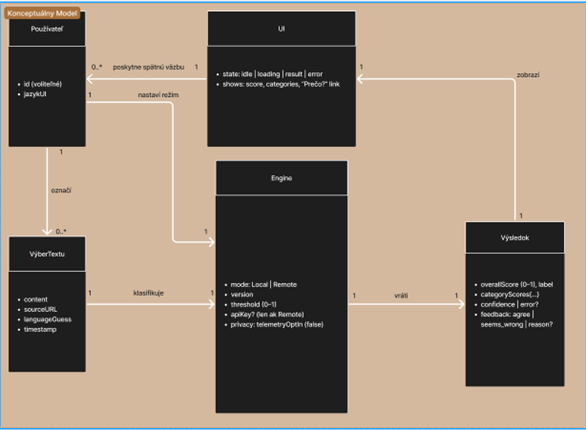
\includegraphics[width=0.82\linewidth,height=0.50\textheight,keepaspectratio]{figures/Konceptual}
  \caption{Konceptuálny model rozšírenia.}
  \label{fig:conceptual_model_ttd}
\end{figure}

Tento konceptuálny model bol použitý ako základ pre návrh architektúry, používateľského rozhrania a toku dát medzi jednotlivými časťami rozšírenia.

\subsection{Architektúra rozšírenia}
Architektúra riešenia vychádza z modelu rozšírení Chrome Manifest V3. Tento model prirodzene rozdeľuje funkcionalitu medzi content script, service worker a používateľské rozhranie rozšírenia. Každá z týchto častí má jasne definovanú úlohu.

\subsubsection{Content script}
Content script je komponent vložený do webovej stránky. V navrhovanom riešení zabezpečuje najmä:
\begin{itemize}
  \item získanie textu vybraného používateľom,
  \item výber textových blokov vhodných na automatickú analýzu,
  \item odoslanie textu na klasifikáciu,
  \item prijatie výsledkov inferencie,
  \item vizuálne označenie alebo rozmazanie toxického obsahu.
\end{itemize}

Content script musí byť navrhnutý tak, aby zbytočne nezaťažoval stránku. Pri automatickom skenovaní preto nemá analyzovať celý DOM bez obmedzení, ale iba vhodné textové prvky spĺňajúce dĺžkové a viditeľnostné kritériá.

\subsubsection{Service worker}
Service worker predstavuje koordinačný prvok rozšírenia. V prostredí Manifest V3 nahrádza pôvodné trvalé background pages a pracuje udalostne. V návrhu zabezpečuje:
\begin{itemize}
  \item prijímanie požiadaviek od používateľského rozhrania a content scriptu,
  \item rozhodovanie o použití lokálneho alebo vzdialeného režimu,
  \item sprostredkovanie komunikácie medzi komponentmi,
  \item vyvolanie opätovného skenovania stránky po zmene nastavení,
  \item správu akcií dostupných cez kontextové menu rozšírenia.
\end{itemize}

Keďže service worker nemá priamy prístup k DOM stránke, všetky operácie nad webovým obsahom musia byť delegované na content script. Tým sa zachováva bezpečnostný model rozšírenia a zároveň sa jasne oddeľuje práca so stránkou od globálnej logiky doplnku.

\subsubsection{Používateľské rozhranie}
Používateľské rozhranie je navrhnuté ako kombinácia rýchleho popup okna, obrazovky nastavení a prekrytia priamo na stránke. Popup slúži na rýchle zobrazenie stavu ochrany, počtu detegovaných prvkov a základných akcií. Obrazovka nastavení poskytuje priestor na podrobnejšiu konfiguráciu, napríklad výber aktívnych kategórií, prísnosti detekcie, režimu inferencie alebo whitelistu domén. Prekrytie na stránke umožňuje pracovať priamo s označeným obsahom.

\subsection{Návrh režimov inferencie}
Jedným z hlavných návrhových rozhodnutí je podpora dvoch režimov inferencie: lokálneho a vzdialeného. Tento hybridný prístup umožňuje vyvážiť požiadavky na súkromie, kvalitu klasifikácie a technickú realizovateľnosť.

\subsubsection{Lokálny režim}
V lokálnom režime prebieha klasifikácia priamo v prehliadači používateľa. Model je súčasťou rozšírenia alebo je načítaný ako jeho lokálny artefakt. Text preto nie je potrebné odosielať na externý server.

Výhodou lokálneho režimu je vyššia úroveň súkromia, nezávislosť od vzdialenej služby a rýchla odozva pri použití optimalizovaného modelu priamo v prehliadači. Nevýhodou je nižšia klasifikačná presnosť v porovnaní s výkonnejším vzdialeným modelom, najmä pri menej zastúpených kategóriách.

\subsubsection{Vzdialený režim}
Vo vzdialenom režime rozšírenie odošle text na vlastný backend alebo proxy API, ktoré zabezpečí klasifikáciu pomocou vzdialeného modelu. Tento režim je vhodný v prípadoch, keď je potrebná vyššia presnosť alebo jednoduchšie experimentovanie s rôznymi modelmi bez nutnosti meniť klientsku časť rozšírenia. Rýchlosť vzdialeného režimu závisí od konkrétneho nasadenia backendu, použitého hardvéru, veľkosti modelu a sieťovej latencie. V testovanom prostredí bolo API spustené lokálne na výkonnom notebooku, preto bola odozva vzdialeného režimu blízka lokálnemu režimu.

Proxy vrstva zároveň chráni citlivé údaje, pretože API kľúče nie sú uložené v klientskom kóde rozšírenia. Okrem toho môže zabezpečiť jednotný formát odpovede, obmedzenie dĺžky vstupu, limitovanie požiadaviek a meranie latencie.

\subsubsection{Prepínanie medzi režimami}
Prepínanie medzi režimami môže byť realizované manuálne používateľom v nastaveniach alebo podmienene podľa jazyka a dostupnosti lokálneho modelu. Z návrhového hľadiska je vhodné, aby bol lokálny režim predvolený a vzdialený režim sa použil len vtedy, keď ho používateľ povolí alebo keď je potrebný pre konkrétny scenár.

Takýto prístup podporuje zásadu \textit{privacy-by-default}, pretože text sa mimo zariadenia neposiela automaticky bez jasnej potreby alebo nastavenia používateľom.

\subsection{Návrh toku dát}
Spracovanie textu v rozšírení prebieha ako postupnosť krokov medzi používateľským rozhraním, content scriptom, service workerom a inferenčnou vrstvou.

Typický scenár manuálnej kontroly vybraného textu pozostáva z nasledujúcich krokov:
\begin{enumerate}
  \item Používateľ označí text na webovej stránke.
  \item Content script získa označený text a pripraví požiadavku na analýzu.
  \item Požiadavka sa odošle príslušnej časti rozšírenia podľa zvoleného režimu.
  \item Inferenčná vrstva vykoná klasifikáciu textu.
  \item Výsledok sa vráti späť content scriptu.
  \item Content script zobrazí výsledok alebo vizuálne označí analyzovaný text.
\end{enumerate}

Pri automatickom skenovaní stránky je proces podobný, ale namiesto jedného vybraného textu sa pracuje s množinou textových úsekov. Aby sa znížila záťaž stránky, návrh počíta s obmedzením počtu analyzovaných prvkov, dávkovým spracovaním, cache výsledkov a filtrovaním nerelevantných DOM prvkov.

\subsection{Návrh práce s kategóriami toxicity a prahmi}
Keďže detekcia toxicity je problém viacnásobnej klasifikácie, systém nemá poskytovať iba jedno binárne rozhodnutie. Každý analyzovaný text môže patriť do viacerých kategórií súčasne, napríklad všeobecná toxicita, urážka, obscénnosť, hrozba alebo nenávisť voči identite.

Výsledok klasifikácie by preto mal obsahovať:
\begin{itemize}
  \item hlavný verdikt, či ide o potenciálne toxický obsah,
  \item skóre pre jednotlivé kategórie,
  \item informáciu o tom, ktoré kategórie prekročili nastavené prahy,
  \item voliteľné upozornenie pri nižšej spoľahlivosti výsledku.
\end{itemize}

Prahy detekcie nemusia byť rovnaké pre všetky kategórie. Napríklad hrozby môžu vyžadovať citlivejší prah než všeobecná toxicita. Preto návrh počíta s internými prahmi pre jednotlivé kategórie a s používateľským nastavením prísnosti, ktoré tieto prahy upravuje jednoduchým a zrozumiteľným spôsobom.

\subsection{Bezpečnostné a súkromnostné opatrenia}
Bezpečnosť a ochrana súkromia patria medzi hlavné kritériá návrhu. Systém preto uplatňuje tieto zásady:
\begin{itemize}
  \item lokálne spracovanie je preferovaný režim,
  \item vzdialené spracovanie je používateľovi zreteľne signalizované,
  \item API kľúče sa neukladajú v klientskom kóde,
  \item rozšírenie nepoužíva vzdialene hostovaný vykonateľný kód,
  \item analyzujú sa iba relevantné textové časti stránky,
  \item uchováva sa len nevyhnutné minimum nastavení a spätnej väzby.
\end{itemize}

Takýto návrh je v súlade s technickými obmedzeniami Manifest V3 a zároveň podporuje princípy minimalizácie údajov a transparentnosti voči používateľovi.

\section{Prototypovanie používateľského rozhrania}
Používateľské rozhranie doplnku \textit{Toxic Text Detector} bolo navrhované iteratívne formou prototypovania v dvoch hlavných iteráciách. Cieľom rozhrania bolo umožniť používateľovi rýchlo rozpoznať potenciálne toxické časti online diskusií, pričom zásah do čítania mal zostať čo najmenší. Dôležitou požiadavkou bola aj reverzibilita akcií, pretože používateľ musí mať možnosť označený text kedykoľvek zobraziť alebo opätovne skryť.

Prvá iterácia vznikla ako interaktívny prototyp vo Figme. Slúžila najmä na overenie rozloženia obrazoviek, pomenovania prvkov a základných interakčných vzorov, ako je rozmazanie toxického textu, odhalenie obsahu, otvorenie vysvetlenia a prístup k nastaveniam. Druhá iterácia bola vytvorená ako bežiaci HTML/React prototyp pomocou technológií Vite a React. Táto verzia už lepšie približovala správanie finálneho rozšírenia, najmä popup okno, stránku nastavení a prekrytie priamo na webovej stránke.

\subsection{UX výskum}
UX výskum sa zameral na situáciu, v ktorej používateľ prehliada verejné diskusie alebo dlhšie vlákna komentárov. V takomto prostredí je dôležité, aby ochrana nevyžadovala zložité rozhodovanie pri každom komentári. Používateľ má byť chránený pred nechceným obsahom, ale zároveň má mať možnosť zobraziť si text v prípade potreby, napríklad pri moderovaní alebo pri posudzovaní kontextu diskusie.

Z návrhového hľadiska boli sledované najmä tieto otázky:
\begin{itemize}
  \item Ako môže rozhranie signalizovať toxicitu bez zbytočného prerušenia čítania?
  \item Ako zachovať akcie reverzibilné, aby používateľ nestratil kontrolu nad obsahom?
  \item Aké minimum vysvetlenia je potrebné, aby používateľ výsledku detekcie rozumel?
  \item Ako sprístupniť nastavenia tak, aby boli dostupné, ale nie rušivé?
\end{itemize}

Na základe analýzy potrieb boli identifikované dve typické skupiny používateľov:
\begin{itemize}
  \item \textbf{Bežný používateľ:} chce rýchlo prehliadať diskusie bez zbytočných zásahov do čítania.
  \item \textbf{Moderátor alebo správca komunity:} potrebuje obsah zobraziť aj v prípade ochrany, no zároveň chce jasné označenie rizikových častí.
\end{itemize}

\subsection{Návrh sekvencií obrazoviek}
Návrh toku obrazoviek bol postavený okolo kontinuálnej slučky prehliadania:
\textit{čítať} $\rightarrow$ \textit{detegovať} $\rightarrow$ \textit{voliteľne odhaliť} $\rightarrow$ \textit{pochopiť dôvod} $\rightarrow$ \textit{upraviť nastavenia} $\rightarrow$ \textit{pokračovať v čítaní}.

Interakcia je ukotvená priamo v zozname komentárov, zatiaľ čo globálna konfigurácia je dostupná cez popup rozšírenia a obrazovku nastavení. Na zníženie interakčných nákladov používa UI rovnaký štrukturálny vzor naprieč obrazovkami: jasnú hlavičku, jednu primárnu obsahovú oblasť a obmedzenú množinu akcií.

Základné obrazovky a akcie sú znázornené na obrázku~\ref{fig:screen_sequence_proto2}. Tento návrh bol použitý ako podklad pre implementáciu bežiaceho HTML/React prototypu.

\begin{figure}[htbp]
  \centering
  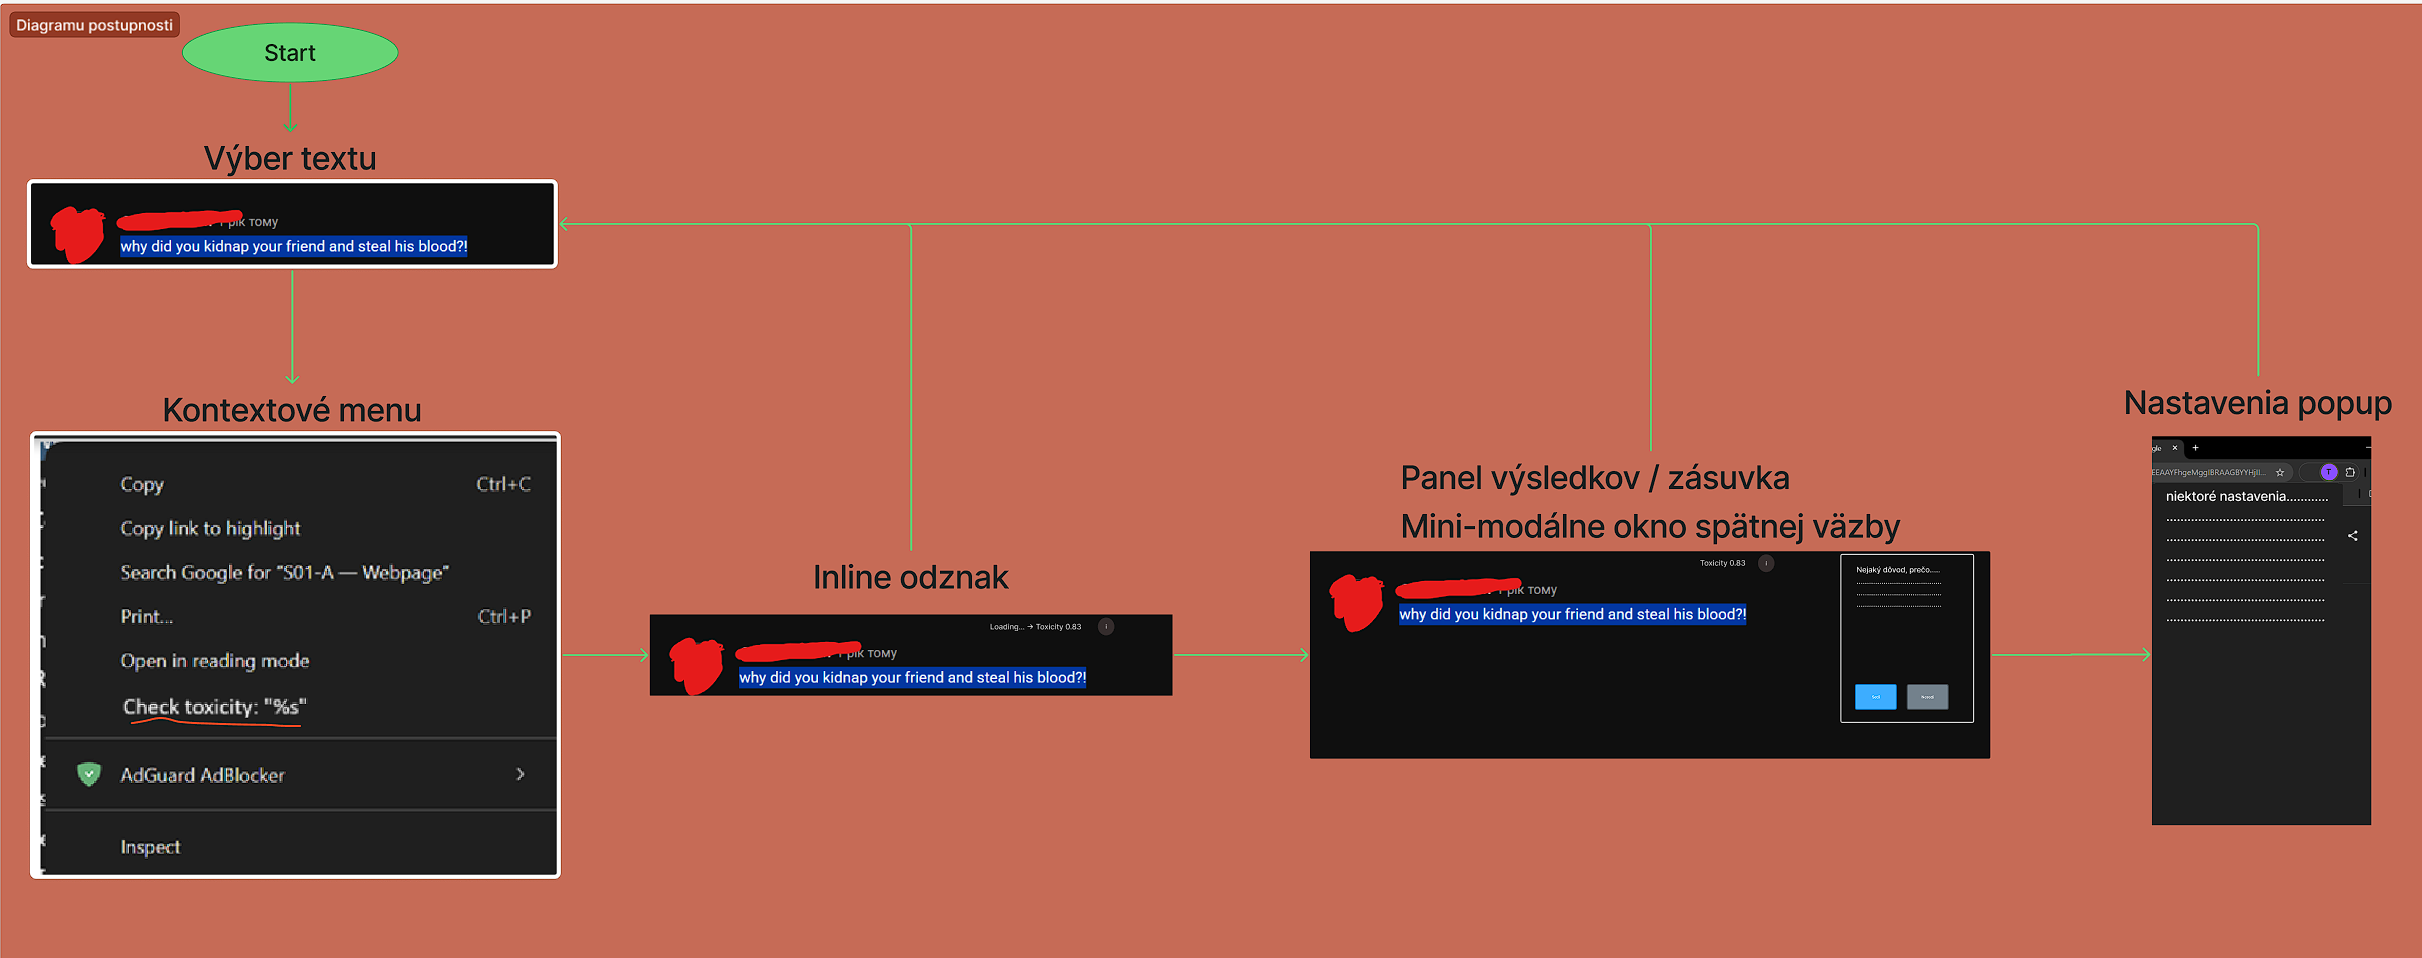
\includegraphics[width=0.90\linewidth,height=0.55\textheight,keepaspectratio]{figures/Sekv}
  \caption{Návrh postupností obrazoviek a navigácie rozšírenia.}
  \label{fig:screen_sequence_proto2}
\end{figure}

Navrhnuté boli najmä tieto časti používateľského rozhrania:
\begin{itemize}
  \item \textbf{Prekrytie na stránke:} toxické komentáre sú predvolene rozmazané, ak je zapnuté automatické rozmazanie.
  \item \textbf{Ovládanie na úrovni komentára:} používateľ môže text zobraziť alebo skryť a otvoriť vysvetlenie dôvodu označenia.
  \item \textbf{Popup rozšírenia:} zobrazuje stav ochrany, počet aktívnych kategórií a základné metriky aktivity.
  \item \textbf{Nastavenia:} umožňujú zapnúť alebo vypnúť kategórie, upraviť prísnosť detekcie a spravovať whitelist domén.
\end{itemize}

\subsection{Prototypy používateľského rozhrania}
Prvý prototyp bol vytvorený vo Figme ako interaktívny mock-up so strednou vernosťou. Jeho cieľom bolo overiť mentálny model a základný interakčný vzor bez implementačných detailov, najmä rozmazanie toxického textu, zobrazenie a skrytie na úrovni komentára, prístup k nastaveniam a jednoduché mini-modálne okno spätnej väzby. Mini-modálne okno spätnej väzby zostalo iba súčasťou skorého návrhu používateľského rozhrania. Do finálnej implementácie rozšírenia nebolo zahrnuté, pretože prvé riešenie nepôsobilo dostatočne použiteľne a jeho dopracovanie by si vyžadovalo samostatný návrh, ukladanie dát a ďalšie testovanie.

\begin{figure}[htbp]
  \centering
  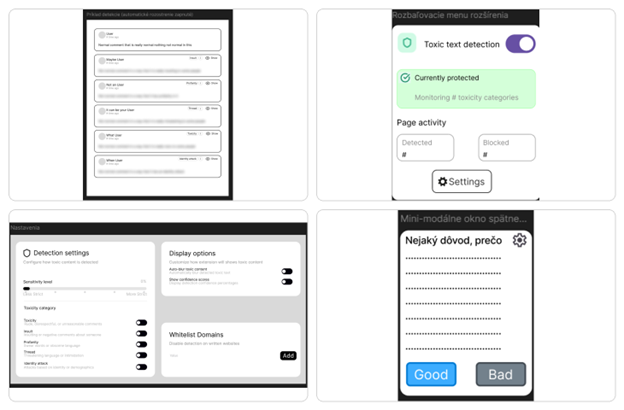
\includegraphics[width=0.90\linewidth,height=0.55\textheight,keepaspectratio]{figures/Prot1}
  \caption{Prvý prototyp vo Figme.}
  \label{fig:prototype1_figma}
\end{figure}

Druhý prototyp implementoval overený interakčný vzor v bežiacom HTML/React prototype. Táto iterácia zvýšila fidelitu návrhu a zabezpečila, že všetky prepínače a stavy sa správajú konzistentne: globálne zapnutie ochrany, automatické rozmazanie, zapnutie a vypnutie kategórií a voliteľné zobrazenie confidence skóre. Stav bol centralizovaný cez kontext nastavení, aby popup, obrazovka nastavení a karty komentárov na stránke vždy reflektovali rovnakú konfiguráciu.

\begin{figure}[htbp]
  \centering
  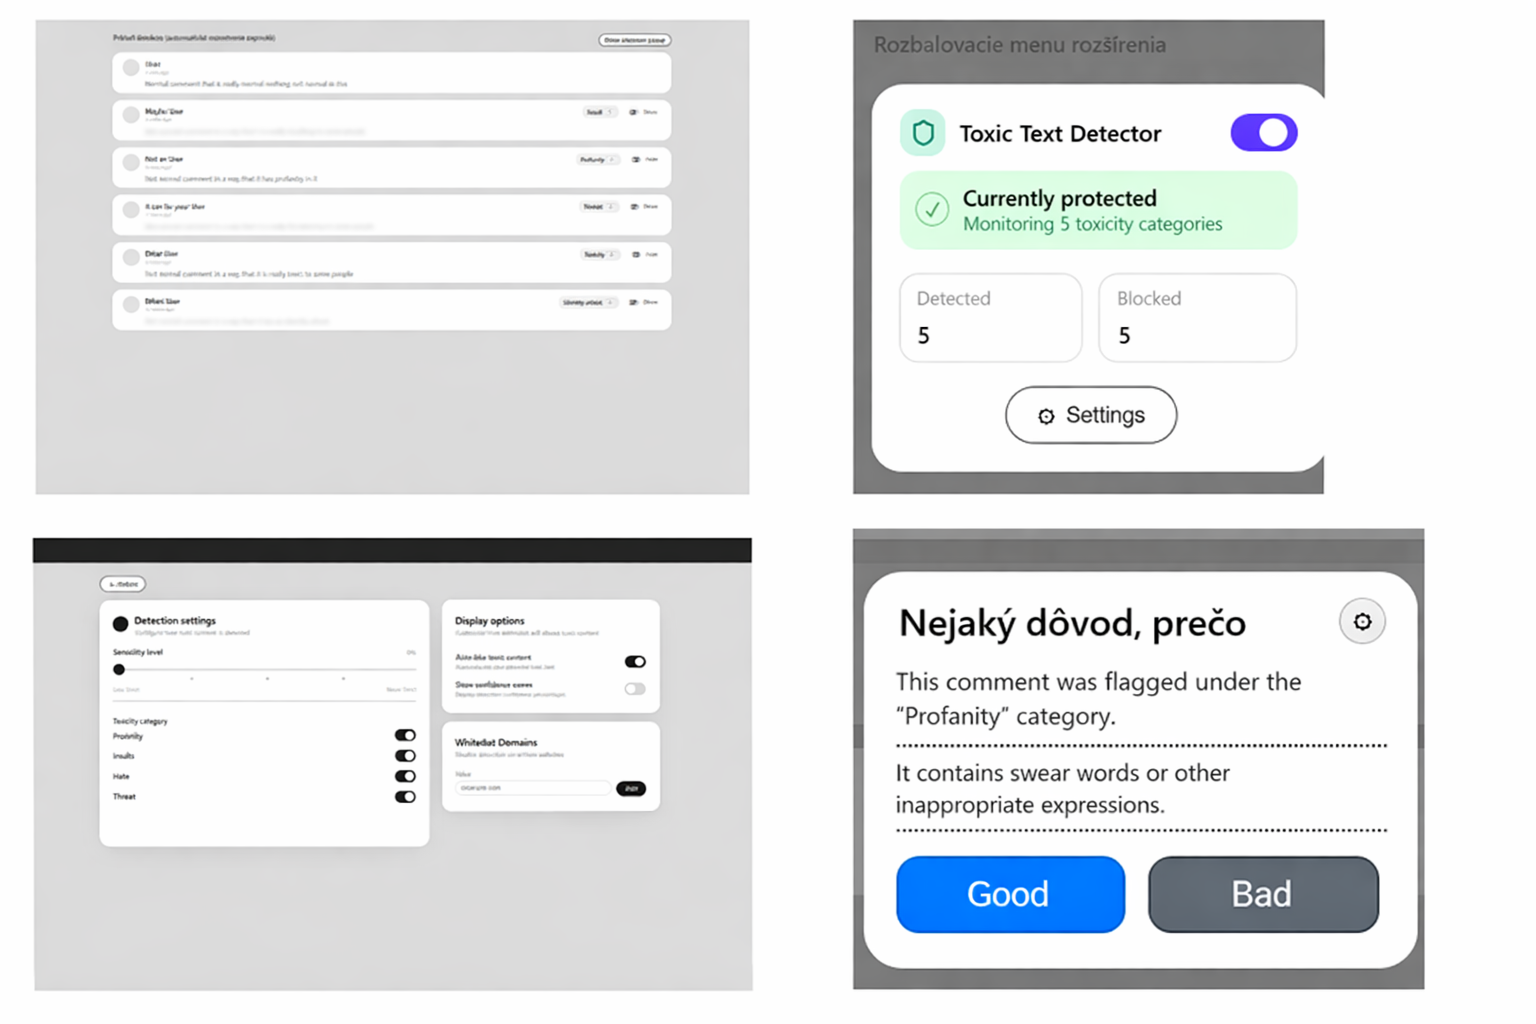
\includegraphics[width=0.90\linewidth,height=0.55\textheight,keepaspectratio]{figures/Prot2}
  \caption{Ukážka implementovaného rozhrania v druhom prototype.}
  \label{fig:prototype2_react}
\end{figure}

Pre potreby dokumentácie sú uvedené aj odkazy na zdroje návrhu:
\begin{itemize}
  \item Zdrojový súbor prototypu: \href{https://www.figma.com/design/To6xEq40ptUYcN36ClJxXR/UX-2-Stakhov-Vladysav?node-id=0-1&t=iu2xqZT8ewasfSXn-1}{Figma Design File}.
  \item Interaktívny náhľad prototypu: \href{https://www.figma.com/design/To6xEq40ptUYcN36ClJxXR/UX-2-Stakhov-Vladysav?node-id=0-1&t=iu2xqZT8ewasfSXn-1}{Figma Prototype}.
  \item Detailný popis, testovacie scenáre a výsledky: \href{https://www.figma.com/board/uDsfPT4P9LXAWeYCLPSIT0/UX-3-Stakhov-Vladysav?node-id=0-1&p=f&t=pL4GL526mWDMBFQd-0}{FigJam -- Prototypovanie a testovanie}.
\end{itemize}

\subsection{Zmeny na základe prototypovania}
Na základe priebežných zistení počas návrhu boli realizované tieto kľúčové zmeny:
\begin{itemize}
  \item \textbf{Zlepšenie vizuálnej hierarchie v kartách komentárov:} zvýraznenie hlavičky a zníženie vizuálnej dominance sekundárnych informácií.
  \item \textbf{Presun kontextových akcií do hlavičky karty:} rýchlejšia objaviteľnosť ovládania, napríklad reveal/hide a vysvetlenia dôvodu označenia.
  \item \textbf{Funkčné prepínače kategórií:} vypnutie kategórie okamžite upraví správanie detekcie a rozmazania pre daný typ toxicity.
  \item \textbf{Zjednotenie stavov v celom UI:} popup, nastavenia a prekrytie na stránke vždy zobrazujú tú istú konfiguráciu.
  \item \textbf{Jasnejší systém stavov:} chránený stav využíva výraznejšiu status kartu, zatiaľ čo vypnutý stav používa neutrálnejší vizuál.
\end{itemize}

Kompletný zdrojový kód prototypu je dostupný v repozitári:
\begin{itemize}
  \item \textbf{GIT projekt:} \href{https://git.kpi.fei.tuke.sk/vs800ru/ux3-vladyslav-stakhov}{git.kpi.fei.tuke.sk}.
\end{itemize}

\section{Implementácia rozšírenia}
Výsledná implementácia rozšírenia \textit{Toxic Text Detector} pozostáva zo štyroch hlavných častí: konfiguračnej vrstvy rozšírenia, používateľského rozhrania vytvoreného v Reacte, background logiky vo forme service workera a content scriptu, ktorý vykonáva lokálnu detekciu toxicity priamo na stránke.

Konfigurácia rozšírenia je definovaná v súbore \emph{manifest.json}. Použitý je formát Chrome Manifest V3, v ktorom je ako service worker zaregistrovaný súbor \emph{background.js}. Manifest zároveň určuje popup okno \emph{popup.html}, stránku nastavení \emph{options.html}, content scripty a web-accessible resources potrebné pre TensorFlow.js a WASM backend.

Používateľské rozhranie rozšírenia je implementované v priečinku \emph{src}. Popup rozhranie sa inicializuje cez súbor \emph{popupMain.jsx}, stránka nastavení cez \emph{optionsMain.jsx}. Obe časti používajú spoločný kontext \emph{SettingsContext.jsx}, ktorý zabezpečuje jednotnú prácu s nastaveniami a ich uloženie do synchronizovaného úložiska prehliadača.

Samotná lokálna detekcia toxicity je implementovaná v súbore \emph{contentScript.js}. Tento súbor obsahuje načítanie modelu, výber kandidátnych textových uzlov, klasifikáciu textu, prácu s cache a vizuálne označovanie toxického obsahu na stránke. Background skript \emph{background.js} vytvára kontextové menu a sprostredkúva komunikáciu medzi popup rozhraním a content scriptom aktívnej karty.

\subsection{Build proces a konfigurácia}
Build proces bol realizovaný pomocou nástroja Vite. Konfigurácia v súbore \emph{vite.config.js} definuje dva vstupné body: \emph{popup.html} a \emph{options.html}. Pri produkčnom zostavení sa tak generujú dve samostatné HTML stránky rozšírenia, pričom každá načítava svoj vlastný React vstupný bod.

Súbor \emph{popup.html} načítava skript \emph{popupMain.jsx}, zatiaľ čo \emph{options.html} načítava súbor \emph{optionsMain.jsx}. Popup rozhranie a stránka nastavení sa preto zostavujú nezávisle, ale stále používajú spoločné komponenty a zdieľaný stav.

Závislosti projektu sú definované v súbore \emph{package.json}. Pre používateľské rozhranie sú použité knižnice React a React DOM. Lokálna inferencia využíva TensorFlow.js, model Toxicity a WASM backend. Produkčný build sa vytvára príkazom \emph{npm run build}.

Manifest deklaruje používanie Manifest V3, service worker \emph{background.js}, popup okno rozšírenia, stránku nastavení, content scripty a web-accessible resources. V rámci content scriptov sa načítavajú knižnice pre jadro TensorFlow.js, konverziu modelu, backendy WASM a CPU, model \emph{toxicity.min.js}, pomocný kontrakt \emph{toxicityContract.global.js} a hlavná implementácia \emph{contentScript.js}. Web-accessible resources obsahujú najmä WASM súbory a priečinok s kernelmi, ktoré TensorFlow.js potrebuje pri lokálnom behu modelu.

\subsection{Implementácia popup rozhrania}
Popup rozhranie je inicializované v súbore \emph{popupMain.jsx}. Tento súbor vytvára React koreň, obalí popup komponent do \emph{SettingsProvider} a pomocou hooku \emph{useTabStats} priebežne načítava štatistiky z aktívnej karty.

Komponent \emph{PopupRoot} získava zo stavového kontextu informáciu o tom, či je rozšírenie zapnuté, a zároveň z hooku \emph{useTabStats} načítava počty detegovaných a zablokovaných prvkov. Po kliknutí na prepínač ochrany sa zavolá funkcia \emph{toggleEnabled()} a následne sa background skriptu odošle správa pre opätovné skenovanie aktívnej karty. Tým sa vyžiada nové skenovanie aktuálnej stránky.

Samotný vizuál popup okna je implementovaný v komponente \emph{ExtensionPopup.jsx}. Tento komponent prijíma všetky potrebné dáta cez props: stav ochrany, callback na jej prepnutie, callback na otvorenie nastavení, počet aktívnych kategórií a štatistiky z aktuálnej stránky. Popup zobrazuje hlavnú kartu so stavom ochrany, prepínač, dva informačné bloky s počtom detegovaných a blokovaných prvkov a tlačidlo pre otvorenie nastavení. Štýly popup okna sú definované v súbore \emph{popup.css}.

\subsection{Implementácia stránky nastavení}
Stránka nastavení sa inicializuje v súbore \emph{optionsMain.jsx}. Rovnako ako popup rozhranie používa \emph{SettingsProvider}, takže všetky zmeny nastavení sú zapisované do rovnakého dátového modelu.

Hlavným komponentom tejto časti je \emph{SettingsLayout.jsx}. Tento komponent používa hodnoty a funkcie zo súboru \emph{SettingsContext.jsx} a vykresľuje ich vo forme viacerých kariet rozdelených podľa typu nastavení. Implementácia obsahuje posuvník citlivosti detekcie, prepínače jednotlivých kategórií toxicity, prepínač automatického rozmazania toxického textu, prepínač zobrazenia confidence skóre, formulár pre pridanie domény do whitelistu, tlačidlo na reset nastavení, export a import nastavení vo formáte JSON a tlačidlo na manuálne opätovné skenovanie aktívnej karty.

Pri zmene citlivosti alebo pri prepnutí niektorej kategórie komponent okamžite volá funkciu \emph{pingRescan()}, ktorá odošle background skriptu správu pre opätovné skenovanie aktívnej karty. Takto sa zmena nastavenia okamžite prejaví aj na otvorenej stránke bez potreby ručného obnovenia karty. Štýly tejto časti sú definované v súbore \emph{settings.css}.

\subsection{Správa nastavení a perzistencia}
Zdieľaný stav rozšírenia je implementovaný v súbore \emph{SettingsContext.jsx}. Tento súbor definuje konštantu \emph{DEFAULT\_SETTINGS}, ktorá obsahuje predvolený stav ochrany, citlivosť, nastavenia zobrazenia, aktívne kategórie toxicity a whitelist domén.

Po inicializácii \emph{SettingsProvider} sa z úložiska načíta uložený objekt nastavení. Ak nastavenia v úložisku neexistujú, použijú sa predvolené hodnoty. Po každej zmene stavu sa aktualizovaná konfigurácia uloží späť.

Kontext zároveň poskytuje funkcie \emph{toggleEnabled()}, \emph{setSensitivity()}, \emph{toggleAutoBlur()}, \emph{toggleShowConfidence()}, \emph{toggleCategory()}, \emph{addWhitelist()} a \emph{removeWhitelist()}, ktoré používajú popup a stránka nastavení. Normalizácia domén je implementovaná pomocnou funkciou \emph{normalizeDomain()}, ktorá odstraňuje protokol, cestu a prefix \emph{www}. Táto funkcia sa používa pri ukladaní whitelistu, aby sa rôzne zápisy tej istej domény neukladali ako odlišné hodnoty.

\subsection{Background logika a komunikácia}
Service worker rozšírenia je implementovaný v súbore \emph{background.js}. Táto časť nepracuje s DOM stromom stránky, ale zabezpečuje centrálne akcie rozšírenia a komunikáciu s content scriptom.

Pri inštalácii a štarte rozšírenia sa vytvárajú tri položky kontextového menu: kontrola vybraného textu na toxicitu, skenovanie stránky na toxicitu a odstránenie existujúcich označení toxicity. Po kliknutí na niektorú z týchto položiek service worker vyhľadá aktívnu kartu a odošle jej správu cez rozhranie kariet, čím spustí príslušnú akciu v content scripte.

Background skript zároveň spracúva správy od popup rozhrania. Pri požiadavke na získanie štatistík najprv zistí aktívnu kartu a potom od content scriptu vyžiada štatistiky stránky. Pri požiadavke na opätovné skenovanie aktívnej karty odošle content scriptu správu na nové skenovanie stránky. Takto popup rozhranie získa údaje o stránke bez priameho prístupu k DOM.

Keďže background skript v MV3 nemá priamy prístup k obsahu stránky, všetky akcie nad obsahom musia byť delegované na content script. Tento model sa používa pri kontrole vybraného textu, pri skenovaní celej stránky aj pri odstraňovaní existujúcich označení.

\section{Implementácia lokálnej inferencie toxicity}

Táto časť sa venuje lokálnemu spracovaniu textu priamo v prostredí prehliadača. Opisuje načítanie modelu, normalizáciu výstupu, klasifikáciu textových úsekov, prácu s cache a spôsob vizuálneho označovania toxického obsahu na webovej stránke. Lokálna inferencia je dôležitou súčasťou riešenia, pretože podporuje ochranu súkromia používateľa a znižuje závislosť od vzdialených služieb.

\subsection{Načítanie modelu a normalizácia výstupu}
Lokálny model je načítavaný v content scripte funkciou \emph{loadToxicityModel()}. Implementácia používa premennú \emph{modelPromise}, aby sa model nenačítaval opakovane pri každej klasifikácii. Po prvom zavolaní sa vytvorený prísľub znovu používa pri ďalších požiadavkách.

Funkcia najprv nastaví cestu k WASM súboru pomocou rozhrania TensorFlow.js, pričom cesta sa generuje cez runtime API rozšírenia. Následne sa systém pokúsi aktivovať backend \emph{wasm}. Ak inicializácia zlyhá, použije sa fallback na backend \emph{cpu}.

Po úspešnej inicializácii backendu sa načíta model toxicity, pričom zoznam štítkov obsahuje kategórie \emph{toxicity}, \emph{severe toxicity}, \emph{obscene}, \emph{insult}, \emph{threat} a \emph{identity attack}. Prahová hodnota modelu je pri načítaní nastavená na nulovú hodnotu, pretože konečné rozhodovanie o toxicite sa nerobí priamo na úrovni predvoleného prahu modelu, ale cez vlastnú logiku implementovanú v súbore \emph{toxicityContract.global.js}.

Súbor \emph{toxicityContract.global.js} implementuje pomocnú vrstvu medzi surovým výstupom modelu a logikou rozšírenia. Definuje zoznam štítkov, základné prahové hodnoty, funkcie pre normalizáciu požiadavky, normalizáciu skóre, úpravu prahov podľa používateľskej prísnosti a výpočet finálneho verdiktu. Najdôležitejšou časťou je funkcia, ktorá z prijatých skóre vytvorí jednotný objekt odpovede obsahujúci režim detekcie, názov modelu, normalizované skóre, aplikované prahy, výsledný verdikt, spustené kategórie a latenciu klasifikácie.

Používateľské rozhranie pracuje s kategóriami \textit{Toxicity}, \textit{Insult}, \textit{Profanity}, \textit{Threat} a \textit{Identity attack}. Tieto kategórie sa v content scripte mapujú na konkrétne modelové štítky pomocou funkcie \emph{buildContractSettingsFromUI()}. Rovnako sa tu prevádza používateľská hodnota \emph{sensitivity} na interný parameter \emph{strictness}, ktorý sa následne použije pri úprave prahov.

\subsection{Klasifikácia textu a práca s cache}
Hlavná logika klasifikácie je implementovaná v súbore \emph{contentScript.js}. Súbor definuje limity pre minimálnu a maximálnu dĺžku textu, maximálny počet kandidátnych textových uzlov, veľkosť dávky pri klasifikácii a veľkosť LRU cache.

Pri manuálnej kontrole vybraného textu sa používa funkcia \emph{handleCheckSelection()}. Tá najprv načíta aktuálne nastavenia, overí, či je rozšírenie zapnuté a či doména nie je vo whiteliste. Potom získa text aktuálneho výberu pomocou funkcie \emph{getSelectedText()}. Ak text spĺňa dĺžkové obmedzenia, odošle sa na klasifikáciu cez funkciu \emph{classifySingleText()}.

Pri plnom skenovaní stránky sa najprv cez funkciu \emph{collectPageCandidateTextNodes()} vyberú vhodné textové uzly z DOM stromu. Do spracovania sa nezaraďujú prvky ako \emph{script}, \emph{style}, \emph{input}, \emph{textarea} alebo už označené časti textu. Zohľadňuje sa aj minimálna dĺžka textu a viditeľnosť prvku vo viewport priestore. Ak stránka prekročí definovaný limit počtu kandidátov alebo objemu textu, používateľ dostane upozornenie, že plný lokálny scan nie je vhodný a má použiť kontrolu len vybraného textu.

Samotná dávková klasifikácia je implementovaná vo funkcii \emph{classifyTextNodes()}. Texty sa najprv normalizujú, potom sa porovnajú s cache a unikátne texty sa rozdelia do dávok s definovanou veľkosťou. Na každú dávku sa následne zavolá klasifikačná funkcia, ktorá spracuje výstup modelu a vráti jednotnú odpoveď podľa interného kontraktu rozšírenia.

Na obmedzenie opakovaných výpočtov bola implementovaná vlastná LRU cache cez funkciu \emph{createLRU()}. Cache uchováva výsledky klasifikácie pre konkrétny text a konkrétnu kombináciu aktívnych štítkov a prísnosti. Pri zmene nastavení v synchronizovanom úložisku sa cache automaticky vymaže, aby sa staré výsledky nepoužívali po zmene citlivosti alebo aktívnych kategórií.

\subsection{Vizuálne označenie toxického obsahu}
Po detekcii toxického textu content script upravuje DOM stránky priamo. Funkcia \emph{createMarkerFromTextNode()} nahradí pôvodný textový uzol vlastným prvkom \emph{span} s interným atribútom rozšírenia. Vo vnútri tohto elementu sa vytvorí textový prvok, blur efekt a toolbar alebo inline chip s kategóriou a skóre.

Ak je v nastaveniach aktívne automatické rozmazanie, text dostane príslušnú blur triedu. Používateľ môže kliknutím na tento text blur efekt zapnúť alebo vypnúť. Tým sa zachováva reverzibilita interakcie bez potreby opätovného načítania stránky.

Tooltip a informačný chip sa vytvárajú pomocou funkcie \emph{createToolbarElement()}, ktorá zoberie primárnu kategóriu výsledku a confidence skóre. Štýly všetkých týchto prvkov sa vkladajú dynamicky cez funkciu \emph{injectStyles()}, ktorá do dokumentu pridáva vlastný štýlový prvok. Odstránenie existujúcich značiek toxicity zabezpečuje funkcia \emph{clearTTDDecorations()}, ktorá prejde všetky aktívne označené prvky, odstráni pomocné toolbar prvky a obnoví pôvodný text stránky.

\section{Vzdialený režim inferencie cez API}
Popri lokálnom režime je v projekte pripravený aj vzdialený režim inferencie, určený pre scenáre, kde je výhodnejšie použiť výkonnejší model mimo prehliadača. Ide napríklad o viacjazyčné spracovanie, experimenty s iným modelom alebo porovnanie presnosti a latencie.

Rozšírenie v tomto režime neposiela požiadavky priamo na externého poskytovateľa, ale komunikuje s vlastným minimálnym backendom, teda proxy API. Tento backend poskytuje jednotné rozhranie \emph{/predict}, autorizáciu cez Bearer token, obmedzenia vstupu, napríklad maximálnu dĺžku textu, a meranie latencie.

Výstup API má stabilnú štruktúru pozostávajúcu z per-label skóre, výsledného verdiktu a meta-informácií. Vďaka tomu môže používateľské rozhranie pracovať s rovnakým formátom dát bez ohľadu na to, či výsledok pochádza z lokálneho alebo vzdialeného režimu. Proxy vrstva zároveň chráni API kľúče, keďže sa nenachádzajú v klientskom kóde rozšírenia.

\section{Doplňujúce mechanizmy implementácie}

Okrem hlavnej logiky detekcie toxicity obsahuje rozšírenie aj viacero doplnkových mechanizmov, ktoré zlepšujú použiteľnosť, kontrolu používateľa a prehľad o stave systému. Medzi tieto mechanizmy patrí whitelist domén a získavanie štatistík z aktívnej stránky.

\subsection{Whitelist domén}
Whitelist domén je spravovaný v používateľskom rozhraní cez komponent \emph{SettingsLayout.jsx}. Domény možno pridávať cez vstupné pole a odstraňovať cez tlačidlo pri každej položke zoznamu.

V content scripte sa whitelist používa cez funkciu \emph{domainIsWhitelisted()}. Pri otvorení stránky alebo pri zmene nastavení content script porovná aktuálny host s normalizovaným zoznamom domén. Ak je doména vo whiteliste, detekcia sa nevykoná a existujúce označenia sa odstránia cez funkciu \emph{clearTTDDecorations()}.

\subsection{Získavanie štatistík z aktívnej stránky}
Na zobrazovanie údajov v popup okne je implementovaný hook \emph{useTabStats.js}. Tento hook periodicky posiela background skriptu požiadavku na získanie štatistík. Background následne vyžiada od content scriptu aktuálne štatistiky stránky.

Content script vracia údaje cez funkciu \emph{getCurrentStats()}, ktorá spočíta počet označených textových úsekov, počet momentálne rozmazaných úsekov, počet aktívnych kategórií, poslednú vykonanú akciu, poslednú stavovú správu a informáciu, či práve prebieha klasifikácia. Tieto údaje sa v popup okne zobrazujú ako activity metriky.

\section{Praktické obmedzenia implementácie}
Počas implementácie sa ukázalo, že lokálna detekcia toxicity v rozšírení prehliadača je realizovateľná, ale vyžaduje technické obmedzenia. Najmä pri väčších stránkach nie je vhodné analyzovať celý DOM bez filtrov a limitov. Preto boli pridané obmedzenia počtu kandidátnych textových uzlov, celkovej dĺžky textu a dĺžky manuálne vybraného úseku.

Ďalším praktickým obmedzením je prostredie Chrome Manifest V3. Service worker je udalostne riadený a nemusí zostať trvalo aktívny. Z tohto dôvodu bolo potrebné navrhnúť komunikáciu tak, aby dôležité operácie nad obsahom stránky vykonával content script a aby stav rozšírenia bol uchovávaný v perzistentnom úložisku.

Medzi obmedzenia finálnej implementácie patrí aj absencia plnohodnotného mechanizmu spätnej väzby používateľa pri nesprávnej klasifikácii. Tento prvok bol v zadaní uvedený ako voliteľné rozšírenie a bol zvažovaný v skorom návrhu používateľského rozhrania, avšak nebol zahrnutý do finálnej verzie rozšírenia. Dôvodom bolo, že prvý návrh spätnej väzby nepôsobil dostatočne použiteľne a jeho dopracovanie by si vyžadovalo ďalšie návrhové rozhodnutia, spôsob ukladania údajov, ochranu súkromia a samostatné testovanie.

\section{Príprava experimentálneho overenia}
Aby bolo možné overiť funkčnosť a kvalitu riešenia, praktická časť počíta s viacerými úrovňami testovania: funkčným testovaním, výkonnostným testovaním, testovaním používateľskej skúsenosti a hodnotením kvality klasifikácie.

Na overenie správania rozšírenia a použitých modelov boli pripravené pomocné testovacie skripty a experimentálne postupy. Ich cieľom nebolo tvoriť samostatnú funkcionalitu rozšírenia, ale umožniť opakovateľné meranie vlastností, ktoré boli definované v cieľoch práce a následne vyhodnotené v samostatnej kapitole.

Testovacie časti boli zamerané najmä na overenie správania lokálneho modelu, porovnanie backendov pri lokálnej inferencii, meranie klasifikačných metrík na validačných dátach a kontrolu vplyvu rozhodovacích prahov. Pri používateľskom rozhraní boli pripravené scenáre úloh, ktoré umožnili overiť zrozumiteľnosť interakcií, reverzibilitu rozmazania a použiteľnosť nastavení.

Výsledky týchto testov nie sú uvádzané v praktickej časti, pretože sú súčasťou kapitoly venovanej vyhodnoteniu riešenia.

\section{Zhrnutie praktickej časti}
Praktická časť predstavila návrh a implementáciu rozšírenia prehliadača \textit{Toxic Text Detector}. Riešenie je založené na Chrome Manifest V3 a pozostáva z používateľského rozhrania, content scriptu, service workera, vrstvy perzistentných nastavení a inferenčného mechanizmu.

V kapitole boli najskôr definované funkčné a nefunkčné požiadavky, následne bol opísaný konceptuálny model a architektúra riešenia. Osobitná pozornosť bola venovaná hybridnému modelu inferencie, ktorý kombinuje lokálne spracovanie textu s možnosťou vzdialeného režimu cez API. Lokálny režim podporuje ochranu súkromia a pri optimalizovanom modeli poskytuje rýchlu odozvu priamo v prehliadači, zatiaľ čo vzdialený režim vytvára priestor pre presnejšie modely a jednoduchšiu experimentálnu výmenu inferenčnej logiky.

Ďalšia časť kapitoly sa venovala prototypovaniu používateľského rozhrania. Boli opísané dve iterácie návrhu: Figma prototyp a následný HTML/React prototyp. Tieto prototypy pomohli overiť hlavné interakčné princípy, ako je rozmazanie toxického textu, možnosť odhalenia obsahu, zobrazenie dôvodu označenia a konfigurácia kategórií.

Implementačná časť opísala konkrétne komponenty rozšírenia, build proces, prácu s nastaveniami, background logiku, lokálnu inferenciu pomocou TensorFlow.js, cache výsledkov, vizuálne označovanie toxického obsahu a doplnkové mechanizmy, ako je whitelist domén a získavanie štatistík z aktívnej stránky. Zároveň boli pomenované praktické obmedzenia riešenia, najmä výkonové limity pri lokálnej analýze väčších stránok a jazykové obmedzenie použitého lokálneho modelu.

Navrhnuté a implementované riešenie tak vytvára základ pre overenie funkčnosti, používateľskej skúsenosti a kvality klasifikácie v ďalšej časti práce.
\chapter{Vyhodnotenie riešenia}

Táto kapitola sa venuje vyhodnoteniu navrhnutého a implementovaného riešenia \textit{Toxic Text Detector}. Hodnotenie je rozdelené na viacero častí, ktoré spoločne posudzujú používateľské rozhranie, vzdialený režim inferencie, lokálny TF.js model a optimalizovaný lokálny model. Cieľom kapitoly je overiť, do akej miery riešenie spĺňa požiadavky definované v predchádzajúcich častiach práce, najmä z hľadiska použiteľnosti, presnosti, výkonu a ochrany súkromia.

\section{Metodika vyhodnotenia}
Vyhodnotenie navrhnutého riešenia bolo realizované na viacerých úrovniach, aby bolo možné posúdiť nielen technickú funkčnosť rozšírenia, ale aj kvalitu používateľského rozhrania a správanie modelov v lokálnom aj vzdialenom režime inferencie. Hodnotenie preto zahŕňa používateľské testovanie prototypov rozhrania, podrobnejšie experimenty so vzdialeným modelom toxicity, orientačné vyhodnotenie pôvodného lokálneho TF.js modelu a vyhodnotenie optimalizovaného lokálneho modelu vo formáte TensorFlow.js GraphModel.

Pri používateľskom rozhraní bolo cieľom overiť zrozumiteľnosť interakcií, objaviteľnosť hlavných ovládacích prvkov a celkové vnímanie použiteľnosti. Hodnotenie prebiehalo formou scenárových úloh, krátkeho post-test dotazníka s 5-bodovou Likertovou škálou, kvalitatívnych pozorovaní typu think-aloud a následného krátkeho rozhovoru.

Pri modelovej časti bolo cieľom vyhodnotiť kvalitu detekcie toxicity pomocou metrík viacštítkovej klasifikácie, pričom rozsah hodnotenia sa líšil podľa konkrétneho režimu a modelu. Pri vzdialenom režime boli podrobnejšie analyzované viaceré verzie modelu, nerovnováha tried a rozhodovacie prahy. Pri lokálnom režime bolo hodnotenie rozdelené na orientačné overenie pôvodného predtrénovaného TF.js modelu a následné vyhodnotenie optimalizovaného lokálneho modelu, ktorý bol použitý ako praktickejší variant pre finálne riešenie.

\section{Vyhodnotenie používateľského rozhrania}

Používateľské rozhranie bolo vyhodnocované v dvoch iteráciách, ktoré zodpovedajú postupnému vývoju prototypu. Prvá iterácia overovala základný mentálny model a hlavné interakčné vzory, zatiaľ čo druhá iterácia sa sústredila na konzistentnosť stavov, použiteľnosť ovládacích prvkov a realistickejšie správanie rozhrania. Vyhodnotenie tejto časti preto porovnáva zistenia z oboch prototypov a ukazuje, ako sa spätná väzba od účastníkov testovania premietla do ďalšieho návrhu.

\subsection{Prvý prototyp a jeho verifikácia}
Prvý prototyp bol vytvorený vo Figme ako interaktívny mock-up so strednou vernosťou. Jeho cieľom bolo overiť mentálny model a základný interakčný vzor bez implementačných detailov: rozmazanie toxického textu, zobrazenie a skrytie na úrovni komentára, prístup k nastaveniam a jednoduché mini-modálne okno spätnej väzby.

\textbf{Metóda verifikácie.} Testovanie prebiehalo formou krátkej moderovanej relácie. Účastníci riešili scenárové úlohy, napríklad zobraziť a opäť skryť rozmazaný komentár, nájsť dôvod alebo kategóriu a zmeniť nastavenie, pričom priebežne verbalizovali svoje rozhodnutia formou think-aloud. Po úlohách vyplnili krátky post-test dotazník s 5-bodovým hodnotením vybraných častí UI, doplnený otvorenými otázkami.

\textbf{Účastníci.} Prvý prototyp bol testovaný s \textbf{5} účastníkmi (n~=~5).

\textbf{Výsledky a interpretácia.}
\begin{itemize}
  \item \textbf{Kvantitatívne:} Interakčný koncept bol hodnotený pozitívne a používanie bolo vnímané ako jednoduché. Najlepšie dopadlo rozbaľovacie menu rozšírenia, kde prevažovali hodnotenia 5/5 a ojedinele 4/5. Príklady detekcie a nastavenia dosiahli mierne nižšie hodnotenia, stále prevažne 4--5/5, avšak s ojedinelým 3/5, čo naznačuje priestor na zlepšenie v jasnosti a spoľahlivosti.
  \item \textbf{Kvalitatívne:} Účastníci oceňovali jednoduchosť prototypu a bezprostrednosť interakcií. Ako najviac pozitívna časť sa najčastejšie uvádzalo rozbaľovacie menu; časť účastníkov vyzdvihla aj nastavenia. Ako najmenej obľúbené sa opakovane objavili príklady detekcie a mini-modálne okno spätnej väzby. Najvýraznejšia negatívna spätná väzba sa týkala ovládania v nastaveniach, najmä poznámok o nefunkčných alebo ťažko použiteľných tlačidlách.
  \item \textbf{Faktory ovplyvnenia:} Malá a potenciálne homogénna vzorka, napríklad prevažne technicky zdatní účastníci, môže viesť k optimistickejším výsledkom. Tento faktor bol zohľadnený pri návrhu zmien pre ďalšiu iteráciu.
\end{itemize}

Podrobná tabuľka výsledkov dotazníka a súhrn pozorovaní sú dostupné v dokumentácii.\footnote{Odkaz na výsledky testovania: \href{https://docs.google.com/spreadsheets/d/1EyIOnNBmjI6_5DjKKHNp1mlViQyInPSu9pmalV57u8U/edit?usp=sharing}{User Testing Results (Spreadsheet)}.}

\subsection{Druhý prototyp a jeho verifikácia}
Druhý prototyp implementoval overený interakčný vzor v bežiacom HTML/React prototype (Vite + React). Táto iterácia zvýšila fidelitu a zabezpečila, že všetky prepínače a stavy sa správajú konzistentne: globálne zapnutie ochrany, správanie Auto-blur, zapnutie alebo vypnutie kategórií a voliteľné zobrazenie istoty.

Verifikácia v druhej iterácii opätovne použila rovnaký typ scenárových úloh, aby bolo možné porovnať zmeny medzi iteráciami. Dotazník bol administrovaný znovu a súhrnné skóre za druhý prototyp je \textbf{86.4/100}.

\textbf{Interpretácia výsledkov.} Oproti prvej iterácii sa zlepšila konzistentnosť stavov a objaviteľnosť ovládacích prvkov, najmä po presune kontextových akcií do hlavičky karty a po zjednotení vizuálnych stavov v celom rozhraní. Výsledky naznačujú, že druhá iterácia lepšie napĺňa požiadavku na rýchlu a reverzibilnú interakciu bez výrazného narušenia čítania.

\textbf{Obmedzenia a faktory ovplyvňujúce výsledky.} Malá alebo homogénna vzorka, napríklad prevažne technicky zdatní účastníci, môže skresliť výsledky hodnotenia. Zároveň druhý prototyp používa simulované výstupy detekcie, čo môže ovplyvniť vnímanú užitočnosť v porovnaní s integráciou reálneho modelu.

\section{Vyhodnotenie vzdialeného režimu inferencie}

Vzdialený režim inferencie bol hodnotený ako alternatíva k lokálnemu spracovaniu textu, ktorá umožňuje použiť výkonnejší model a flexibilnejšie experimentovať s nastavením prahov. Táto časť sa zameriava najmä na vplyv nerovnováhy tried, porovnanie jednotlivých iterácií modelu a rozdiel medzi validačne optimalizovanými a produktovými prahmi. Výsledky slúžia na posúdenie toho, akú úlohu môže vzdialený režim zohrávať v hybridnej architektúre rozšírenia.

\subsection{Nerovnováha tried a príprava dát}
Pri viacštítkovej detekcii toxicity podľa taxonómie Jigsaw sa potvrdila výrazná nerovnováha tried. V baseline rozdelení dát Jigsaw2018 dosahuje napríklad štítok \emph{threat} iba približne 0{,}30\% pozitívnych príkladov v tréningu a 0{,}26\% vo validácii, pričom \emph{severe\_toxic} sa pohybuje približne na úrovni 1\%. Na zlepšenie učenia menšinových tried boli otestované oversampling konfigurácie pre vybrané štítky. Kľúčovým rozhodnutím bolo aplikovať oversampling iba na tréningovú množinu a validačnú množinu ponechať nezmenenú, aby metriky ostali porovnateľné.

\FloatBarrier
\begin{table*}[!htbp]
  \centering
  \small
  \label{tab:jigsaw_imbalance_os}
  \begin{tabularx}{\textwidth}{|p{3.4cm}|p{1.7cm}|Y|Y|Y|Y|Y|Y|}
    \hline
    \textbf{Split} & \textbf{Riadky} & \textbf{toxic} & \textbf{severe} & \textbf{obscene} & \textbf{insult} & \textbf{threat} & \textbf{identity} \\
    \hline
    Baseline (train) & 143\,613 & 9{,}59\% & 1{,}01\% & 5{,}31\% & 4{,}94\% & 0{,}30\% & 0{,}89\% \\
    \hline
    Baseline (val) & 15\,958 & 9{,}56\% & 0{,}90\% & 5{,}18\% & 4{,}88\% & 0{,}26\% & 0{,}83\% \\
    \hline
    Oversampling (train-only, train) & 152\,294 & 14{,}56\% & 4{,}48\% & 9{,}63\% & 9{,}09\% & 2{,}55\% & 2{,}66\% \\
    \hline
    Oversampling (train-only, val) & 15\,958 & \multicolumn{6}{l|}{\emph{nezmenené (identické s Baseline (val))}} \\
    \hline
  \end{tabularx}
  \caption[Rozdelenie pozitívnych príkladov]{Rozdelenie pozitívnych príkladov v Jigsaw2018 (baseline) a po oversamplingu aplikovanom iba na tréningovú množinu.}
\end{table*}
\FloatBarrier

\subsection{Iterácie modelu a porovnanie verzií}
Na pripravených dátach boli vytrénované a vyhodnotené tri iterácie modelu XLM-R, konkrétne verzie v1, v2 a v2\_1, pričom všetky boli hodnotené rovnakým protokolom na validačnej množine Jigsaw2018. Výsledky ukazujú, že verzia v2 dosiahla najlepší kompromis medzi makro-F1, mikro-F1 a Hammingovou stratou a zároveň výrazne zlepšila menšinové triedy. Príkladom je metrika \emph{F1\_threat}, ktorá vzrástla z 0{,}362 na 0{,}743.

\FloatBarrier
\begin{table*}[!htbp]
  \centering
  \small
  \label{tab:xlmr_versions_val}
  \begin{tabularx}{\textwidth}{|Y|Y|Y|Y|Y|Y|}
    \hline
    \textbf{Model} & \textbf{macro-F1} & \textbf{micro-F1} & \textbf{Hamming loss} & \textbf{F1\_threat} & \textbf{F1\_severe} \\
    \hline
    xlmr-toxic-v1 & 0{,}635 & 0{,}777 & 0{,}0169 & 0{,}362 & 0{,}470 \\
    \hline
    xlmr-toxic-v2 & 0{,}780 & 0{,}839 & 0{,}0122 & 0{,}743 & 0{,}628 \\
    \hline
    xlmr-toxic-v2\_1 & 0{,}647 & 0{,}768 & 0{,}0176 & 0{,}448 & 0{,}489 \\
    \hline
  \end{tabularx}
  \caption[Porovnanie verzií XLM-R]{Porovnanie iterácií XLM-R modelu na validačnej množine Jigsaw2018 (multi-label).}
\end{table*}
\FloatBarrier

Verzia v2\_1 bola použitá ako doplnková kontrolná konfigurácia pri experimentoch zameraných na prahovanie a stabilitu správania v produktových nastaveniach rozšírenia.

\subsection{Prahy rozhodovania: tuned vs.\ product}
Keďže ide o multi-label úlohu, nepostačuje jeden globálny prah. Preto boli zavedené per-label prahy v dvoch režimoch: \emph{tuned} prahy optimalizované na validačnej množine a \emph{product} prahy určené pre reálne správanie doplnku, ktoré zohľadňujú aj UX kompromisy. Pri bezpečnostne kritických prejavoch, ako je \emph{threat}, bolo cieľom znížiť počet falošne negatívnych prípadov aj za cenu citlivejšieho rozhodovania.

\FloatBarrier
\begin{table*}[!htbp]
  \centering
  \small
  \label{tab:thresholds_tuned_vs_product}
  \begin{tabularx}{\textwidth}{|Y|Y|Y|}
    \hline
    \textbf{Štítok} & \textbf{tuned} & \textbf{product} \\
    \hline
    toxic & 0{,}675 & 0{,}80 \\
    \hline
    severe\_toxic & 0{,}95 & 0{,}70 \\
    \hline
    obscene & 0{,}89 & 0{,}92 \\
    \hline
    insult & 0{,}85 & 0{,}85 \\
    \hline
    threat & 0{,}945 & 0{,}55 \\
    \hline
    identity\_hate & 0{,}95 & 0{,}75 \\
    \hline
  \end{tabularx}
  \caption[Prahy tuned vs product]{Porovnanie per-label prahov pre režim \emph{tuned} (optimalizácia na val) a \emph{product} (UX kompromis) pre v2\_1.}
\end{table*}
\FloatBarrier

\textbf{Interpretácia.} Výsledky ukazujú, že rozhodovanie modelu je pri menšinových a bezpečnostne citlivých triedach výrazne závislé od nastavenia prahov. Z tohto dôvodu je vhodné oddeľovať prahy optimalizované na validačných dátach od prahov určených pre produktové správanie systému, kde sa okrem klasickej presnosti zohľadňuje aj používateľský dopad falošných pozitív a falošných negatív.

\section{Vyhodnotenie predtrénovaného TF.js toxicity modelu}

Pred návrhom vlastného optimalizovaného lokálneho modelu bol orientačne vyhodnotený aj predtrénovaný model \emph{@tensorflow-models/toxicity}. Tento experiment slúžil ako lokálny baseline a jeho cieľom bolo overiť, či je hotový TF.js model použiteľný pre režim orientovaný na súkromie používateľa. Model nebol použitý ako finálny lokálny režim riešenia, ale poskytol užitočné porovnanie z hľadiska kvality detekcie a výpočtovej náročnosti.

\subsection{Nastavenie experimentu}

Vyhodnotenie bolo vykonané pomocou samostatného Node.js testera, ktorý načítal validačný súbor \emph{val.csv}, spustil predikciu modelu a uložil výsledky do súborov \emph{summary\_metrics.csv}, \emph{per\_label\_metrics.csv}, \emph{predictions.csv}, \emph{config.json} a \emph{run\_log.txt}. Použitá bola verzia \emph{@tensorflow-models/toxicity} 1.2.2 spolu s kompatibilnou verziou TensorFlow.js 1.7.4. Model bol testovaný s backendom \emph{CPU}, globálnym rozhodovacím prahom $\tau = 0{,}85$ a veľkosťou dávky 16.

Keďže praktické lokálne nasadenie rozšírenia nepočítalo so spoľahlivým využitím GPU/WebGL akcelerácie, dôležité bolo najmä správanie modelu v lokálnom režime bez GPU. Toto nastavenie zároveň ukázalo, do akej miery je predtrénovaný TF.js model vhodný pre priebežné spracovanie väčšieho počtu komentárov.

\FloatBarrier
\begin{table*}[!htbp]
  \centering
  \small
  \renewcommand{\arraystretch}{1.15}
  \setlength{\tabcolsep}{4pt}
  \begin{tabularx}{\textwidth}{|P{3.4cm}|Y|Y|Y|Y|Y|}
    \hline
    \textbf{Model} &
    \textbf{Backend} &
    \textbf{TF.js ver.} &
    \textbf{Riadky} &
    \textbf{Prahovanie} &
    \textbf{Batch size} \\
    \hline
    @tensorflow-models/toxicity 1.2.2 &
    CPU &
    1.7.4 &
    15\,958 &
    $\tau=0{,}85$ &
    16 \\
    \hline
    \multicolumn{6}{|P{\dimexpr\textwidth-2\tabcolsep-2\arrayrulewidth\relax}|}{%
      \textbf{Metriky:} macro-F1 = 0{,}279;\quad micro-F1 = 0{,}560;\quad Hamming loss = 0{,}0233;\quad exact match accuracy = 0{,}908.
    } \\
    \hline
    \multicolumn{6}{|P{\dimexpr\textwidth-2\tabcolsep-2\arrayrulewidth\relax}|}{%
      \textbf{Čas:} načítanie modelu = 4{,}76 s;\quad vyhodnotenie = 11\,652{,}35 s;\quad celkový čas = 11\,657{,}22 s; priemerne približne 730 ms na jeden komentár.
    } \\
    \hline
  \end{tabularx}
  \caption[Vyhodnotenie predtrénovaného TF.js toxicity modelu]{Súhrn vyhodnotenia predtrénovaného TF.js toxicity modelu na validačnej množine Jigsaw2018.}
  \label{tab:tfjs_eval_summary}
\end{table*}
\FloatBarrier

\subsection{Výsledky a interpretácia}

Výsledky ukazujú, že model dosahoval najlepšie výsledky pri častejších kategóriách \emph{toxic} a \emph{insult}. Pri štítku \emph{toxic} dosiahol F1 hodnotu 0{,}685 a pri štítku \emph{insult} hodnotu 0{,}603. Pri kategórii \emph{obscene} bola presnosť vysoká, ale návratnosť nízka, čo znamená, že model označoval túto kategóriu opatrne a veľkú časť pozitívnych príkladov neidentifikoval.

Pri zriedkavejších triedach \emph{severe\_toxic}, \emph{threat} a \emph{identity\_hate} model pri zvolenom globálnom prahu neoznačil žiadny pozitívny príklad. Z toho dôvodu bola hodnota F1 pre tieto triedy nulová. Vysoké hodnoty accuracy pri týchto triedach preto nemožno interpretovať ako dôkaz kvalitnej detekcie, keďže sú spôsobené najmä veľkým počtom negatívnych príkladov vo validačných dátach.

\FloatBarrier
\begin{table*}[!htbp]
  \centering
  \small
  \renewcommand{\arraystretch}{1.15}
  \setlength{\tabcolsep}{4pt}
  \begin{tabularx}{\textwidth}{|P{2.8cm}|Y|Y|Y|Y|Y|}
    \hline
    \textbf{Štítok} &
    \textbf{Pozit.} &
    \textbf{Predik. pozit.} &
    \textbf{Precision} &
    \textbf{Recall} &
    \textbf{F1} \\
    \hline
    toxic & 1\,525 & 888 & 0{,}930 & 0{,}542 & 0{,}685 \\
    \hline
    severe\_toxic & 143 & 0 & 0{,}000 & 0{,}000 & 0{,}000 \\
    \hline
    obscene & 826 & 211 & 0{,}948 & 0{,}242 & 0{,}386 \\
    \hline
    insult & 778 & 518 & 0{,}755 & 0{,}503 & 0{,}603 \\
    \hline
    threat & 42 & 0 & 0{,}000 & 0{,}000 & 0{,}000 \\
    \hline
    identity\_hate & 132 & 0 & 0{,}000 & 0{,}000 & 0{,}000 \\
    \hline
  \end{tabularx}
  \caption[Per-label výsledky predtrénovaného TF.js modelu]{Per-label výsledky predtrénovaného TF.js toxicity modelu pri globálnom prahu $\tau = 0{,}85$.}
  \label{tab:tfjs_eval_perlabel}
\end{table*}
\FloatBarrier

Z praktického hľadiska bol najvýraznejším obmedzením čas spracovania. Vyhodnotenie 15\,958 komentárov trvalo viac než tri hodiny, čo zodpovedá približne 730 ms na jeden komentár. Takéto správanie nie je vhodné pre rozšírenie prehliadača, ktoré musí priebežne spracovávať viacero textových uzlov na stránke bez citeľného spomalenia používateľského rozhrania.

Na základe týchto výsledkov nebol predtrénovaný TF.js toxicity model použitý ako finálny lokálny režim. Experiment však ukázal dôležitý baseline: hotový TF.js model poskytuje určitú kvalitu pri častejších kategóriách, ale pri jednom globálnom prahu zlyháva pri menšinových triedach a jeho výpočtová náročnosť je pre praktické lokálne nasadenie príliš vysoká. Toto zistenie motivovalo návrh vlastného optimalizovaného lokálneho modelu, ktorý je opísaný v ďalšej časti.

\section{Vyhodnotenie optimalizovaného lokálneho režimu inferencie}

Po vyhodnotení pôvodného lokálneho baseline modelu bol lokálny režim rozšírený o vlastný optimalizovaný model vo formáte TensorFlow.js GraphModel. Táto časť hodnotí, či takýto model dokáže zlepšiť klasifikačnú kvalitu, zachovať výhody lokálneho spracovania a zároveň dosiahnuť dostatočný výkon pre praktické použitie v rozšírení. Pozornosť je venovaná ladeniu prahov, výsledkom na validačných dátach a porovnaniu backendov CPU a WASM.

\subsection{Nastavenie experimentu}
Táto časť nadväzuje na predchádzajúce experimentálne vyhodnotenie lokálneho TF.js modelu založeného na predtrénovanom balíku toxicity modelu. Pôvodné riešenie slúžilo ako orientačný lokálny baseline, avšak pri jednom globálnom prahu dosahovalo slabšie výsledky najmä pri menšinových triedach. Z tohto dôvodu bol lokálny režim ďalej rozšírený o vlastný model exportovaný do formátu TensorFlow.js GraphModel.

Nový lokálny model pracuje na znakovej reprezentácii vstupu. Každý text je normalizovaný, skrátený na maximálnu dĺžku 256 znakov a následne zakódovaný podľa slovníka znakov. Výstupom modelu je šestica skóre zodpovedajúca taxonómii Jigsaw: \emph{toxic}, \emph{severe\_toxic}, \emph{obscene}, \emph{insult}, \emph{threat} a \emph{identity\_hate}.

Cieľom experimentu bolo overiť dve vlastnosti optimalizovaného lokálneho režimu. Prvou bola klasifikačná použiteľnosť modelu na validačnej množine Jigsaw2018. Druhou bolo porovnanie výkonu backendov \emph{CPU} a \emph{WASM}, keďže lokálna inferencia v rozšírení prehliadača musí byť dostatočne rýchla, aby nespomaľovala používateľské rozhranie. Experiment bol vykonaný na validačnej množine \emph{val.csv} s počtom 15\,958 komentárov. Veľkosť dávky bola nastavená na 64 a použitá verzia TensorFlow.js bola 4.22.0.

\FloatBarrier
\begin{table*}[!htbp]
  \centering
  \small
  \renewcommand{\arraystretch}{1.15}
  \setlength{\tabcolsep}{6pt}
  \begin{tabularx}{\textwidth}{|p{3cm}|Y|Y|Y|Y|Y|}
    \hline
    \textbf{Konfigurácia} &
    \textbf{Model} &
    \textbf{TF.js ver.} &
    \textbf{Riadky} &
    \textbf{Batch size} &
    \textbf{Max. dĺžka vstupu} \\
    \hline
    Optimalizovaný lokálny režim &
    Char-CNN GraphModel &
    4.22.0 &
    15\,958 &
    64 &
    256 znakov \\
    \hline
  \end{tabularx}
  \caption[Nastavenie lokálneho Char-CNN experimentu]{Nastavenie experimentu pre optimalizovaný lokálny režim inferencie pomocou TensorFlow.js GraphModel.}
  \label{tab:local_charcnn_eval_setup}
\end{table*}
\FloatBarrier

\subsection{Ladenie rozhodovacích prahov}
Na rozdiel od pôvodného lokálneho baseline riešenia, ktoré bolo vyhodnotené s jedným globálnym prahom, nový lokálny model používa samostatné rozhodovacie prahy pre jednotlivé štítky. Takéto nastavenie lepšie zodpovedá viacštítkovej povahe úlohy, pretože jednotlivé kategórie toxicity majú rozdielne rozdelenie dát a rozdielnu náročnosť detekcie.

Prahy boli optimalizované na validačnej množine tak, aby sa maximalizovala hodnota F1 pre jednotlivé triedy. Výsledky ukazujú, že model generuje pomerne vysoké skóre pri pozitívnych prípadoch, preto sa najlepšie prahy pohybovali v rozsahu 0{,}90 až 0{,}94.

\FloatBarrier
\begin{table*}[!htbp]
  \centering
  \small
  \renewcommand{\arraystretch}{1.15}
  \begin{tabularx}{\textwidth}{|p{3.2cm}|Y|Y|Y|Y|Y|Y|}
    \hline
    \textbf{Režim} &
    \textbf{toxic} &
    \textbf{severe} &
    \textbf{obscene} &
    \textbf{insult} &
    \textbf{threat} &
    \textbf{identity} \\
    \hline
    Tuned &
    0{,}90 &
    0{,}94 &
    0{,}94 &
    0{,}92 &
    0{,}94 &
    0{,}94 \\
    \hline
    Product &
    0{,}90 &
    0{,}96 &
    0{,}94 &
    0{,}92 &
    0{,}97 &
    0{,}96 \\
    \hline
  \end{tabularx}
  \caption[Prahy pre lokálny Char-CNN model]{Porovnanie per-label prahov pre optimalizovaný lokálny model. Režim \emph{tuned} maximalizuje F1 na validačnej množine, zatiaľ čo režim \emph{product} sprísňuje rozhodovanie pri zriedkavých triedach.}
  \label{tab:local_charcnn_thresholds}
\end{table*}
\FloatBarrier

Režim \emph{product} bol navrhnutý ako konzervatívnejšie nastavenie pre reálne použitie v rozšírení. Pri triedach \emph{severe\_toxic}, \emph{threat} a \emph{identity\_hate} boli prahy zvýšené, pretože tieto triedy majú výrazne menší počet pozitívnych príkladov a pri optimalizácii iba podľa F1 vykazovali nižšiu presnosť. Takéto nastavenie znižuje riziko falošne pozitívneho rozmazania bežného textu.

\subsection{Klasifikačné výsledky na validačnej množine}
Klasifikačné výsledky ukazujú, že model dosahuje najlepšie výsledky pri častejších triedach, najmä \emph{toxic}, \emph{obscene} a \emph{insult}. Najvyššiu hodnotu F1 dosiahol štítok \emph{obscene} s hodnotou 0{,}801. Trieda \emph{toxic} dosiahla F1 0{,}732 a \emph{insult} 0{,}702. Slabšie výsledky boli pozorované pri zriedkavých triedach, hlavne \emph{threat}, kde bolo vo validačnej množine iba 42 pozitívnych príkladov.

\FloatBarrier
\begin{table*}[!htbp]
  \centering
  \small
  \setlength{\tabcolsep}{4pt}
  \begin{tabularx}{\textwidth}{|P{2.6cm}|Y|Y|Y|Y|Y|Y|}
    \hline
    \textbf{Štítok} &
    \textbf{Pozit.} &
    \textbf{Prah} &
    \textbf{Precision} &
    \textbf{Recall} &
    \textbf{F1} &
    \textbf{Accuracy} \\
    \hline
    toxic & 1\,525 & 0{,}90 & 0{,}787 & 0{,}684 & 0{,}732 & 0{,}952 \\
    \hline
    severe\_toxic & 143 & 0{,}94 & 0{,}286 & 0{,}783 & 0{,}419 & 0{,}981 \\
    \hline
    obscene & 826 & 0{,}94 & 0{,}808 & 0{,}794 & 0{,}801 & 0{,}980 \\
    \hline
    insult & 778 & 0{,}92 & 0{,}664 & 0{,}743 & 0{,}702 & 0{,}969 \\
    \hline
    threat & 42 & 0{,}94 & 0{,}189 & 0{,}714 & 0{,}299 & 0{,}991 \\
    \hline
    identity\_hate & 132 & 0{,}94 & 0{,}329 & 0{,}636 & 0{,}434 & 0{,}986 \\
    \hline
  \end{tabularx}
  \caption[Per-label výsledky lokálneho Char-CNN modelu]{Per-label výsledky optimalizovaného lokálneho modelu na validačnej množine Jigsaw2018.}
  \label{tab:local_charcnn_perlabel}
\end{table*}
\FloatBarrier

Okrem samostatných štítkov bol vyhodnotený aj celkový binárny verdikt \emph{toxic}/\emph{non-toxic}, ktorý zodpovedá praktickému správaniu rozšírenia. Text je v používateľskom rozhraní označený alebo rozmazaný vtedy, ak aspoň jeden povolený štítok prekročí nastavený prah. Pri tomto zjednodušenom rozhodovaní dosiahol model F1 0{,}734 pri najlepšom globálnom prahu 0{,}86.

\FloatBarrier
\begin{table*}[!htbp]
  \centering
  \small
  \setlength{\tabcolsep}{4pt}
  \begin{tabularx}{\textwidth}{|P{2.8cm}|Y|Y|Y|Y|Y|Y|}
    \hline
    \textbf{Verdikt} &
    \textbf{Pozit.} &
    \textbf{Prah} &
    \textbf{Precision} &
    \textbf{Recall} &
    \textbf{F1} &
    \textbf{Accuracy} \\
    \hline
    toxic / non-toxic & 1\,623 & 0{,}86 & 0{,}744 & 0{,}725 & 0{,}734 & 0{,}947 \\
    \hline
  \end{tabularx}
  \caption[Celkový toxický verdikt lokálneho modelu]{Vyhodnotenie celkového binárneho verdiktu lokálneho modelu na validačnej množine Jigsaw2018.}
  \label{tab:local_charcnn_overall}
\end{table*}
\FloatBarrier

\textbf{Interpretácia.} Výsledky potvrdzujú, že optimalizovaný lokálny model je výrazne použiteľnejší ako pôvodný lokálny baseline opísaný v predchádzajúcej časti. Zatiaľ čo pôvodný model bol vhodný najmä ako orientačné riešenie typu \emph{privacy-friendly baseline}, nový GraphModel poskytuje skóre pre všetkých šesť štítkov v rovnakej taxonómii ako vzdialený režim a umožňuje samostatné prahovanie pre každú kategóriu. Napriek tomu zostáva detekcia menšinových tried náročná, najmä pre \emph{threat} a \emph{identity\_hate}, kde nízky počet pozitívnych príkladov zvyšuje citlivosť metriky precision na falošne pozitívne predikcie.

\subsection{Porovnanie výkonu backendov CPU a WASM}
Dôležitou súčasťou lokálneho režimu je výkon inferencie. Model bol preto spustený s dvomi backendmi TensorFlow.js: \emph{CPU} a \emph{WASM}. Pri oboch backendch boli klasifikačné metriky rovnaké, rozdiel sa prejavil najmä v rýchlosti výpočtu. Backend \emph{CPU} spracoval 15\,958 komentárov za 85{,}60 s, zatiaľ čo backend \emph{WASM} potreboval 6{,}35 s. Priemerný čas na jeden komentár klesol z 5{,}36 ms na 0{,}40 ms.

\FloatBarrier
\begin{table*}[!htbp]
  \centering
  \small
  \renewcommand{\arraystretch}{1.2}
  \setlength{\tabcolsep}{4pt}
  \begin{tabularx}{\textwidth}{|Y|Y|Y|Y|Y|Y|Y|}
    \hline
    \textbf{Backend} &
    \textbf{Riadky} &
    \textbf{Batch} &
    \textbf{Predikcia [s]} &
    \textbf{Priemer [ms]} &
    \textbf{Priepust. [textov/s]} &
    \textbf{Warm-up [ms]} \\
    \hline
    CPU &
    15\,958 &
    64 &
    85{,}60 &
    5{,}36 &
    186{,}42 &
    34{,}27 \\
    \hline
    WASM &
    15\,958 &
    64 &
    6{,}35 &
    0{,}40 &
    2\,514{,}57 &
    10{,}66 \\
    \hline
  \end{tabularx}
  \caption[Porovnanie CPU a WASM backendu]{Porovnanie výkonu lokálnej inferencie pri backendch CPU a WASM.}
  \label{tab:local_charcnn_backend_perf}
\end{table*}
\FloatBarrier

Backend \emph{WASM} bol približne 13{,}49-krát rýchlejší než backend \emph{CPU} pri samotnej predikcii. Tento rozdiel je prakticky významný, pretože rozšírenie neklasifikuje iba jeden text, ale priebežne skenuje viaceré textové uzly na stránke. Rýchlejšia inferencia znižuje riziko oneskorenia pri prehliadaní obsahu a umožňuje spracovanie väčšieho počtu komentárov bez výrazného dopadu na používateľské rozhranie.

\section{Zhrnutie vyhodnotenia}

Vyhodnotenie ukázalo, že navrhnuté používateľské rozhranie je zrozumiteľné a použiteľné. Druhá iterácia prototypu dosiahla lepšie výsledky než prvá a odstránila viaceré problémy zistené pri prvotnom testovaní.

Z technického hľadiska sa potvrdilo, že lokálny a vzdialený režim inferencie majú rozdielne výhody. Optimalizovaný lokálny režim zachováva princíp \emph{privacy-by-default}, keďže text sa spracúva priamo v prehliadači, a pri použití backendu \emph{WASM} dosahuje dostatočnú rýchlosť na praktické použitie. V porovnaní s pôvodným baseline riešením poskytuje vlastný \emph{GraphModel} lepšiu kontrolu nad prahmi, jednotnejšiu štruktúru výstupu a lepšie možnosti optimalizácie.

Lokálny TF.js model je preto vhodný ako základ pre súkromie orientované nasadenie, avšak pri jednoduchom globálnom prahu dosahuje slabšie výsledky pri menej zastúpených kategóriách. Vzdialený režim naopak umožňuje lepšiu optimalizáciu presnosti, najmä pri menšinových triedach a \emph{per-label} prahovaní.

Navrhnutá hybridná architektúra tak predstavuje vhodný kompromis medzi ochranou súkromia, použiteľnosťou, výkonom a presnosťou detekcie toxického textu.
% !TEX root = ../thesis.tex

\chapter{Záver}

Cieľom tejto záverečnej práce bolo preskúmať možnosti detekcie toxického textu v prostredí webového prehliadača a navrhnúť, implementovať a vyhodnotiť riešenie vo forme rozšírenia \textit{Toxic Text Detector}. Práca sa zamerala na viacštítkovú klasifikáciu toxicity, používateľské rozhranie, ochranu súkromia, architektúru rozšírenia podľa Chrome Manifest V3 a porovnanie lokálneho a vzdialeného režimu inferencie. Výsledkom je funkčný prototyp hybridného systému, ktorý kombinuje spracovanie textu priamo v prehliadači s možnosťou vzdialenej inferencie.

V analytickej časti boli spracované teoretické východiská detekcie toxicity, relevantné datasety, modely, existujúce prístupy a technické aj etické problémy tejto oblasti. Analýza ukázala, že pri návrhu podobného systému nie je rozhodujúca iba presnosť modelu, ale aj spôsob nasadenia, latencia, transparentnosť výsledkov, ochrana súkromia a používateľská dôvera. Na základe týchto poznatkov bolo navrhnuté a implementované rozšírenie pozostávajúce z používateľského rozhrania v Reacte, service workera, content scriptu a vrstvy nastavení uchovávanej v úložisku prehliadača. Rozšírenie umožňuje analyzovať vybraný text alebo textové časti stránky, označiť potenciálne toxický obsah, vizuálne ho rozmazať a poskytnúť používateľovi základné vysvetlenie výsledku pomocou kategórie a skóre.

Dôležitou súčasťou práce bol aj návrh používateľského rozhrania. Rozhranie bolo vytvorené iteratívne, najskôr ako prototyp vo Figme a následne ako bežiaci HTML/React prototyp. Používateľské testovanie ukázalo, že zvolený koncept je zrozumiteľný a používatelia pozitívne vnímali najmä jednoduchosť ovládania, možnosť spätne zobraziť skrytý text a jasné signalizovanie stavu ochrany. Mechanizmus spätnej väzby používateľa pri nesprávnej klasifikácii bol zvažovaný v skorom návrhu, ale keďže išlo o voliteľné rozšírenie a jeho dopracovanie by si vyžadovalo ďalší návrh, ukladanie údajov a samostatné testovanie, nebol zahrnutý do finálnej implementácie.

V oblasti inferencie práca ukázala význam hybridného prístupu. Pôvodne bol ako lokálny variant overený predtrénovaný TF.js model toxicity, no jeho testovanie ukázalo obmedzenia z hľadiska rýchlosti, aktuálnosti a kvality výsledkov pri menej zastúpených kategóriách. Preto bol lokálny režim rozšírený o optimalizovaný TensorFlow.js GraphModel so samostatnými prahmi pre jednotlivé štítky a efektívnejším behom cez WASM backend. Lokálny režim sa ukázal ako rýchly a súkromie zachovávajúci základ, avšak s nižšou presnosťou pri náročnejších kategóriách. Vzdialený režim poskytol priestor pre presnejšiu detekciu a jednoduchšiu výmenu modelu, pričom pri lokálnom spustení API na výkonnom notebooku dosahoval odozvu porovnateľnú s lokálnym režimom. Vyhodnotenie zároveň potvrdilo, že pri detekcii toxicity je vhodné používať samostatné prahy pre jednotlivé kategórie namiesto jedného univerzálneho prahu.

Z pohľadu splnenia cieľov možno konštatovať, že hlavné ciele práce boli splnené. Bola spracovaná analytická časť, navrhnutá architektúra rozšírenia, vytvorené a otestované používateľské rozhranie, implementovaná funkčná verzia rozšírenia pre Chrome Manifest V3 a pripravený lokálny aj vzdialený režim inferencie. Práca zároveň ukázala obmedzenia riešenia, najmä pri detekcii implicitnej, kontextovej a sarkastickej toxicity, pri menej zastúpených kategóriách, pri viacjazyčných textoch a pri dôkladnom hodnotení spravodlivosti modelov. Ďalší vývoj by sa preto mohol zamerať na presnejšiu kalibráciu prahov, rozšírenie vzdialeného režimu o ďalšie modely, lepšie spracovanie rôznych jazykov, používateľskú spätnú väzbu a rozsiahlejšie testovanie na reálnych webových stránkach. Navrhnuté riešenie tak potvrdilo realizovateľnosť prehliadačovo integrovaného nástroja, ktorý vyvažuje presnosť detekcie, používateľskú kontrolu a ochranu súkromia.

%% Bibliography, glossary, acronyms
\backmatter{}


%% -----------------------------------------------------------------
%%                                       _ _
%%       __ _ _ __  _ __   ___ _ __   __| (_) ___ ___  ___
%%      / _` | '_ \| '_ \ / _ \ '_ \ / _` | |/ __/ _ \/ __|
%%     | (_| | |_) | |_) |  __/ | | | (_| | | (_|  __/\__ \
%%      \__,_| .__/| .__/ \___|_| |_|\__,_|_|\___\___||___/
%%           |_|   |_|
%% -----------------------------------------------------------------

\chapter*{\appendixlistname}
\addcontentsline{toc}{chapter}{\appendixlistname}

\begin{description}

   \item[\appendixname{} A] CD médium -- záverečná práca v~elektronickej podobe:
   \begin{itemize}
      \item \textbf{README.md} -- úvodný prehľad repozitára a štruktúry CD média
      \item \textbf{doc} -- záverečná práca vo formáte PDF, systémová príručka, používateľská príručka a obrázky použité v príručkách
      \item \textbf{tex} -- zdrojové súbory záverečnej práce
      \item \textbf{src} -- zdrojové kódy vytvoreného riešenia, rozdelené na frontendovú a backendovú časť
      \item \textbf{bin} -- zostavená verzia rozšírenia pripravená na načítanie do prehliadača
      \item \textbf{pomocné súbory repozitára} -- konfiguračné súbory repozitára a vývojového prostredia, napríklad \textbf{.gitignore} a \textbf{.vscode}
   \end{itemize}

   \item[\autoref{app:system.manual}] \nameref{app:system.manual}
   \item[\autoref{app:user.manual}] \nameref{app:user.manual}

\end{description}

\appendix
\setappendixstyle
\setcounter{chapter}{1}
% !TEX root = ../thesis.tex

\chapter{Systémová príručka}
\label{app:system.manual}

Systémová príručka je súčasťou Git repozitára vo forme súboru \mbox{\textsf{README.md}}. Opisuje technické zloženie, inštaláciu, zostavenie, konfiguráciu a údržbu rozšírenia \textit{Toxic Text Detector}. Je určená najmä pre vývojárov alebo používateľov, ktorí chcú aplikáciu spustiť zo zdrojových súborov, upraviť jej funkcionalitu alebo pokračovať vo vývoji riešenia.

Systémová príručka je dostupná aj online.\footnote{Systémová príručka dostupná online: \url{https://github.com/kkuichi/vs800ru}.}

Projekt je rozdelený na dve hlavné časti. Priečinok \emph{frontend} obsahuje klientsku časť systému vo forme rozšírenia prehliadača Chrome. Priečinok \emph{backend} obsahuje voliteľnú serverovú časť určenú na vzdialenú inferenciu toxicity cez API.

Príručka opisuje štruktúru projektu, použité technológie, lokálny a vzdialený model, zostavenie rozšírenia, načítanie do prehliadača, spustenie API servera, konfiguráciu vzdialeného API a pomocné skripty použité pri hodnotení modelov.
% !TEX root = ../thesis.tex

\chapter{Používateľská príručka}
\label{app:user.manual}

Používateľská príručka je súčasťou Git repozitára. V repozitári je uložená ako súbor \textsf{USER\_MANUAL.md}.\footnote{Používateľská príručka dostupná online: \url{https://github.com/kkuichi/vs800ru/blob/main/docs/USER_MANUAL.md}.}

Príručka je určená pre používateľa alebo hodnotiteľa, ktorý chce rozšírenie \textit{Toxic Text Detector} nainštalovať a používať bez zásahu do zdrojového kódu. Opisuje inštaláciu cez súkromný odkaz v Chrome Web Store alebo manuálne načítanie pripravenej zložky \textsf{dist}.

Ďalej vysvetľuje používanie popup okna, nastavení, kategórií toxicity, automatického rozmazania, skóre istoty, zoznamu povolených domén a režimov lokálneho a vzdialeného spracovania. Súčasťou príručky sú aj odporúčané nastavenia, poznámky k ochrane súkromia, obmedzenia systému a základné riešenie problémov.

% avoid empty lof, lot and lol
\setcounter{figure}{0}
\setcounter{table}{0}
\setcounter{lstlisting}{0}


%% -----------------------------------------------------------------
%%       ___ _   _ _ __ ___   _____   __
%%      / _ \ | | | '__/ _ \ / __\ \ / /
%%     |  __/ |_| | | | (_) | (__ \ V /
%%      \___|\__,_|_|  \___/ \___| \_/
%% -----------------------------------------------------------------

% Životopis autora
% \curriculumvitae\protect
% Táto časť je nepovinná. Autor tu môže uviesť svoje biografické
% údaje, údaje o~záujmoch, účasti na~projektoch, účasti na~súťažiach,
% získané ocenenia, zahraničné pobyty na~praxi, domácu prax, publikácie
% a~pod.

\end{document}
